\documentclass[./main.tex]{subfiles}

\begin{document}
\section{Dataset}
\label{sec:dataset}
To perform the pose estimation in section \ref{sec:pretraining} and section \ref{sec:finetuning}, we need some data on which to train, validate and test our models. The following section describes the datasets that will be used. This starts off in section \ref{sec:ClimbAlong}, where we describe the dataset provided by ClimbAlong. This is then followed by section \ref{sec:dataset_pretraining}, where we describe the datasets that we will be using during pretraining of our models.

\begin{table}[htbp]
    \begin{tabular}{|l|c|c|c|c|}
        \hline
        \textbf{Keypoint label} & \textbf{ClimbAlong} & \textbf{BRACE} & \textbf{Penn Action} \\ \hline
        Head & No & No & Yes \\ \hline
        Nose & Yes & Yes & No \\ \hline
        Left ear & Yes & Yes & No \\ \hline
        Right ear & Yes & Yes & No \\ \hline
        Left eye & No & Yes & No \\ \hline
        Right eye & No & Yes & No \\ \hline
        Left shoulder & Yes & Yes & Yes \\ \hline
        Right shoulder & Yes & Yes & Yes \\ \hline
        Left elbow & Yes & Yes & Yes \\ \hline
        Right elbow & Yes & Yes & Yes \\ \hline
        Left wrist & Yes & Yes & Yes \\ \hline
        Right wrist & Yes & Yes & Yes \\ \hline
        Left pinky & Yes & No & No \\ \hline
        Right pinky & Yes & No & No \\ \hline
        Left index & Yes & No & No \\ \hline
        Right index & Yes & No & No \\ \hline
        Left thumb & Yes & No & No \\ \hline
        Right thumb & Yes & No & No \\ \hline
        Left hip & Yes & Yes & Yes \\ \hline
        Right hip & Yes & Yes & Yes \\ \hline
        Left knee & Yes & Yes & Yes \\ \hline
        Right knee & Yes & Yes & Yes \\ \hline
        Left ankle & Yes & Yes & Yes \\ \hline
        Right ankle & Yes & Yes & Yes \\ \hline
        Left heel & Yes & No & No \\ \hline
        Right heel & Yes & No & No \\ \hline
        Left toes & Yes & No & No \\ \hline
        Right toes & Yes & No & No \\ \hline
    \end{tabular}
    \caption{Overview of the annotated keypoints of the three used datasets}
    \label{tab:keypoints}
\end{table}

\subsection{The Finetuning Dataset}
\label{sec:ClimbAlong}
\begin{figure}[htbp]
    \centering
    \begin{subfigure}{0.3\textwidth}
        \centering
        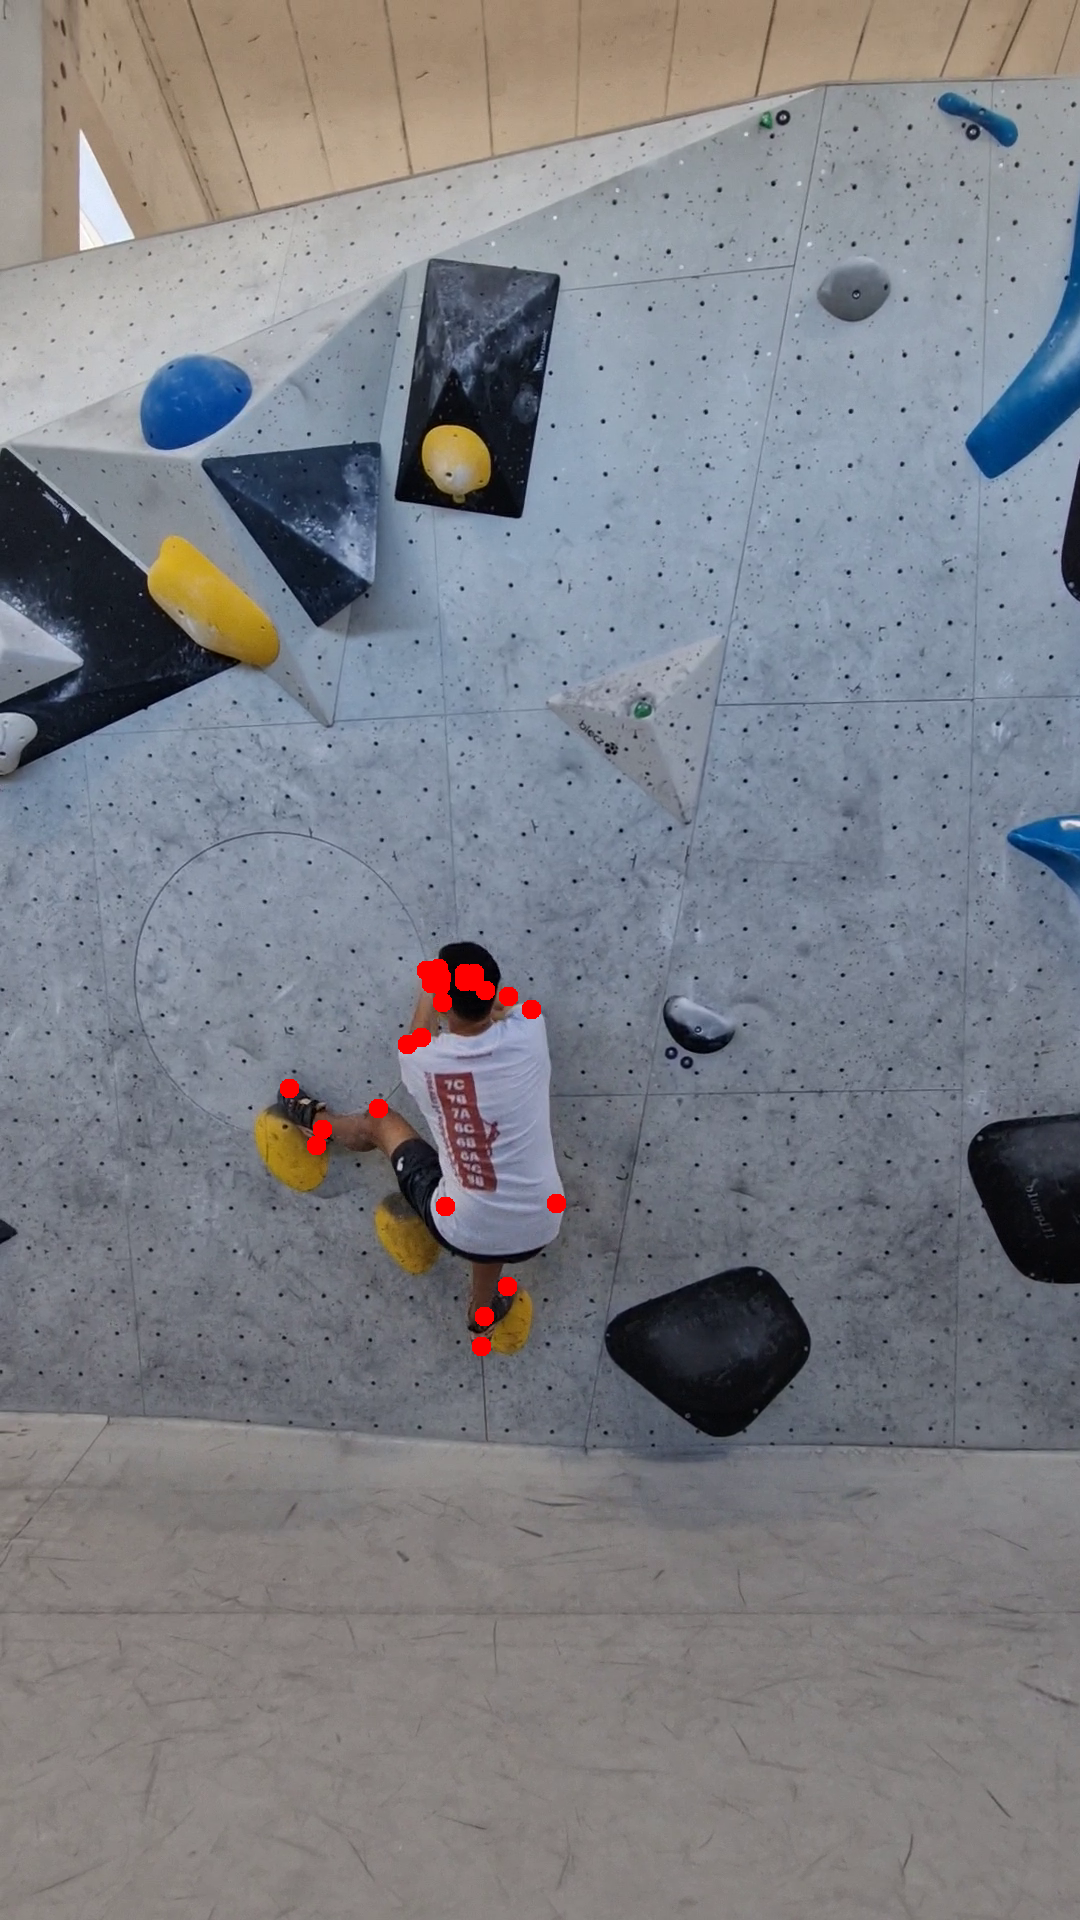
\includegraphics[width=\textwidth]{entities/CA_17.png}
        \caption{Frame 17}
    \end{subfigure}
    \begin{subfigure}{0.3\textwidth}
        \centering
        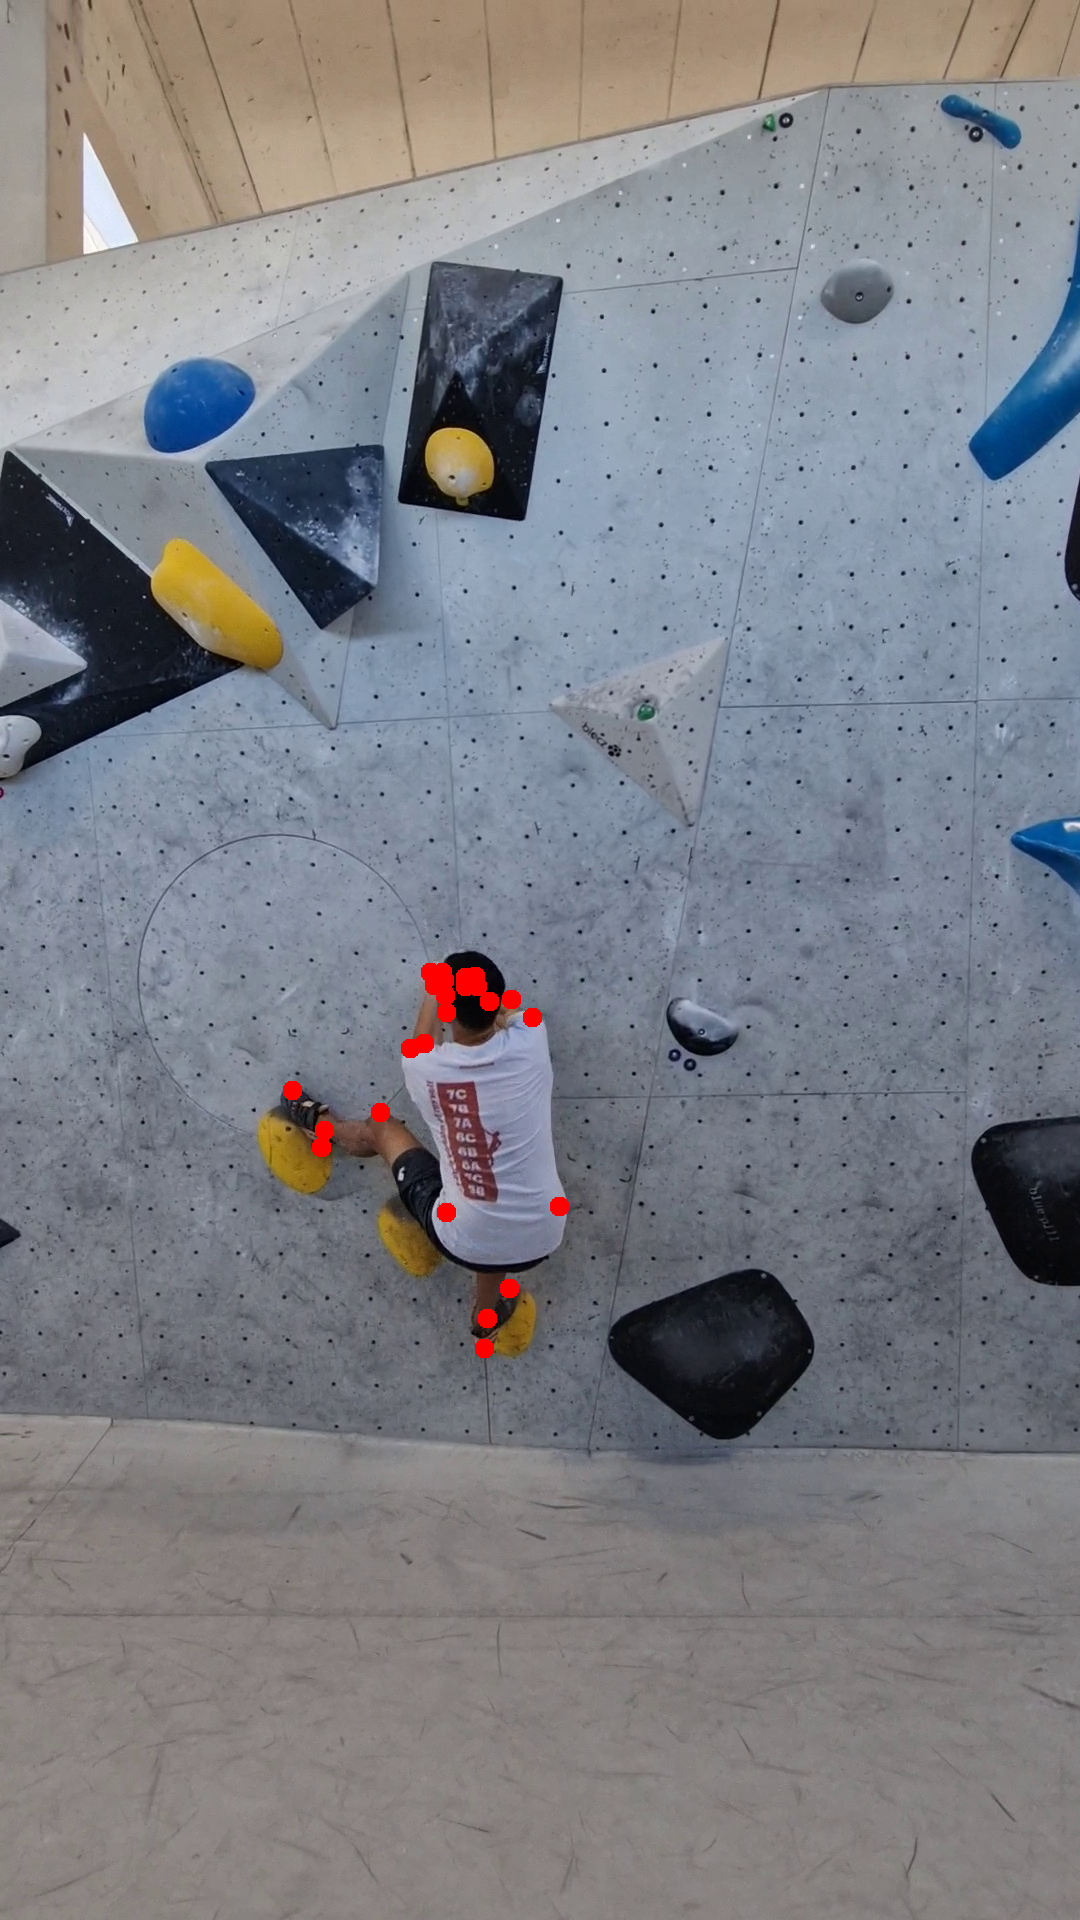
\includegraphics[width=\textwidth]{entities/CA_18.png}
        \caption{Frame 18}
    \end{subfigure}
    \begin{subfigure}{0.3\textwidth}
        \centering
        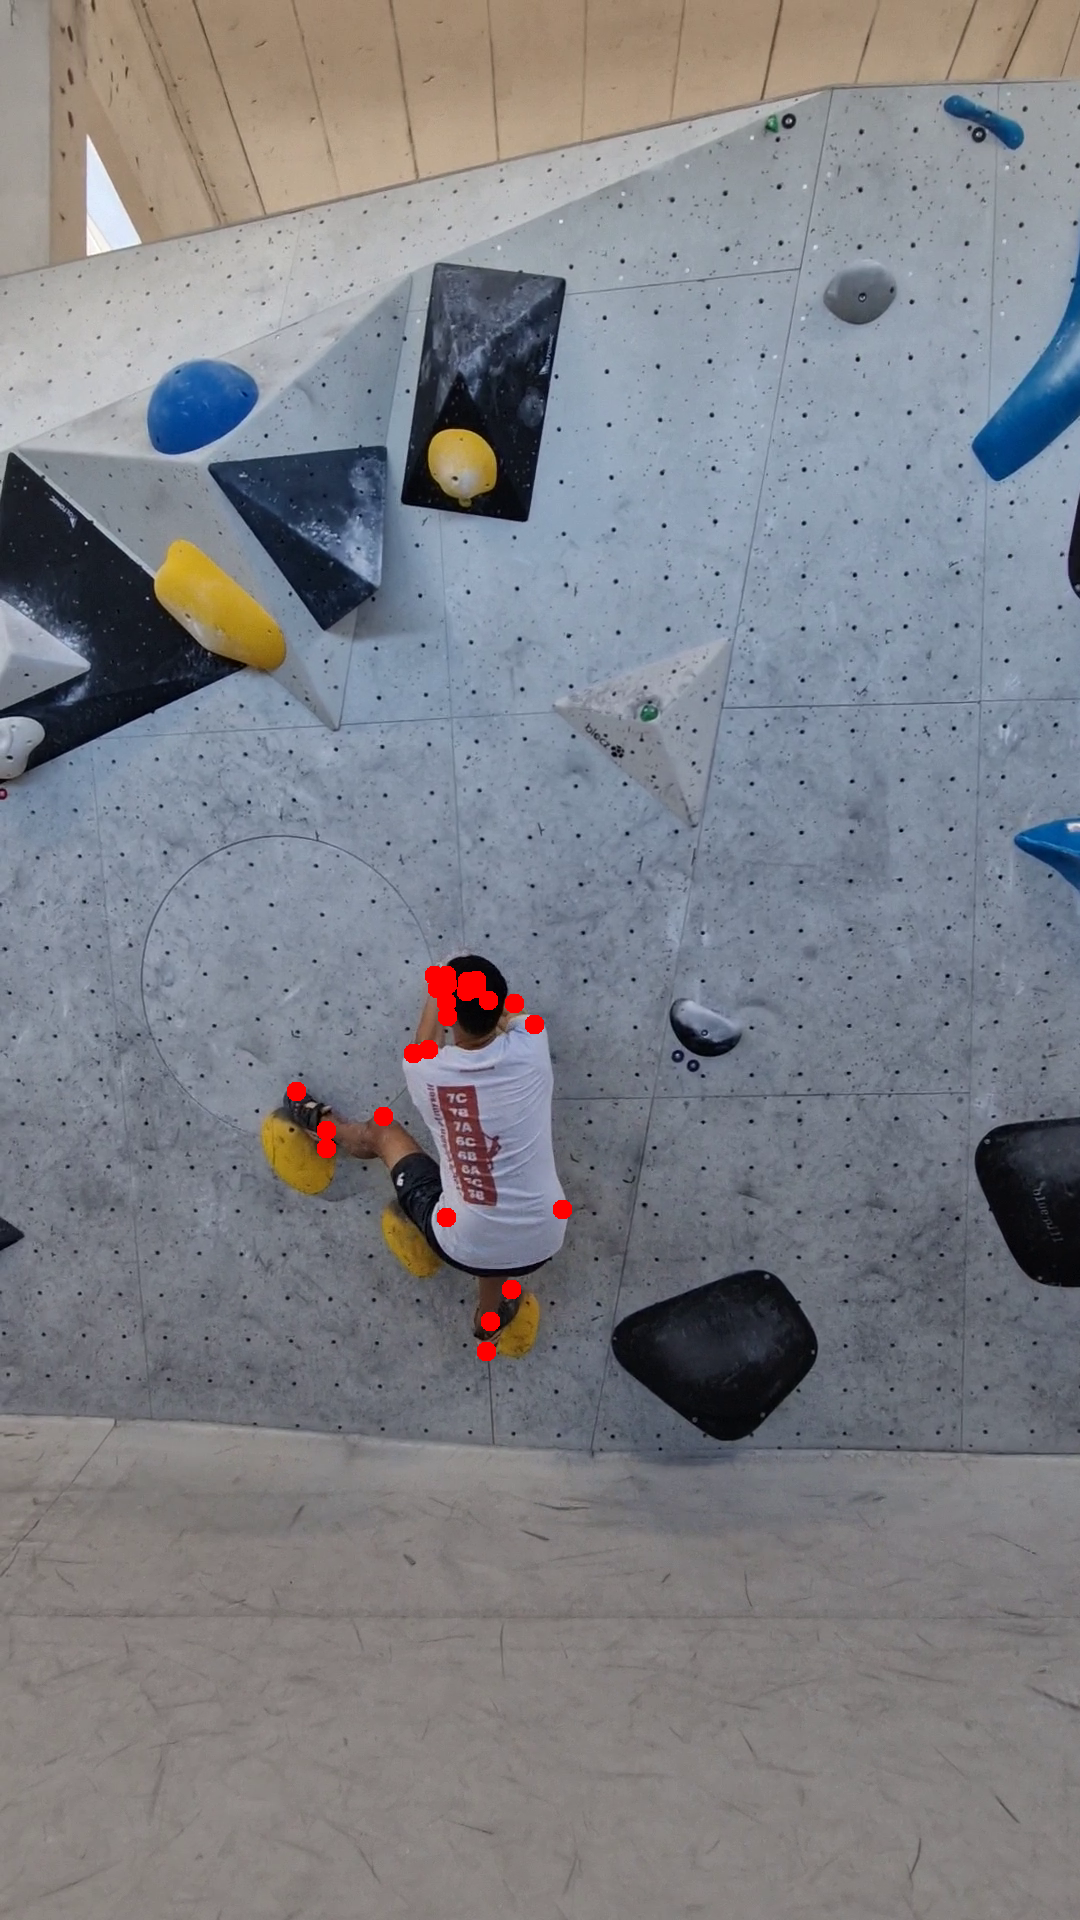
\includegraphics[width=\textwidth]{entities/CA_19.png}
        \caption{Frame 19}
    \end{subfigure}
    \begin{subfigure}{0.3\textwidth}
        \centering
        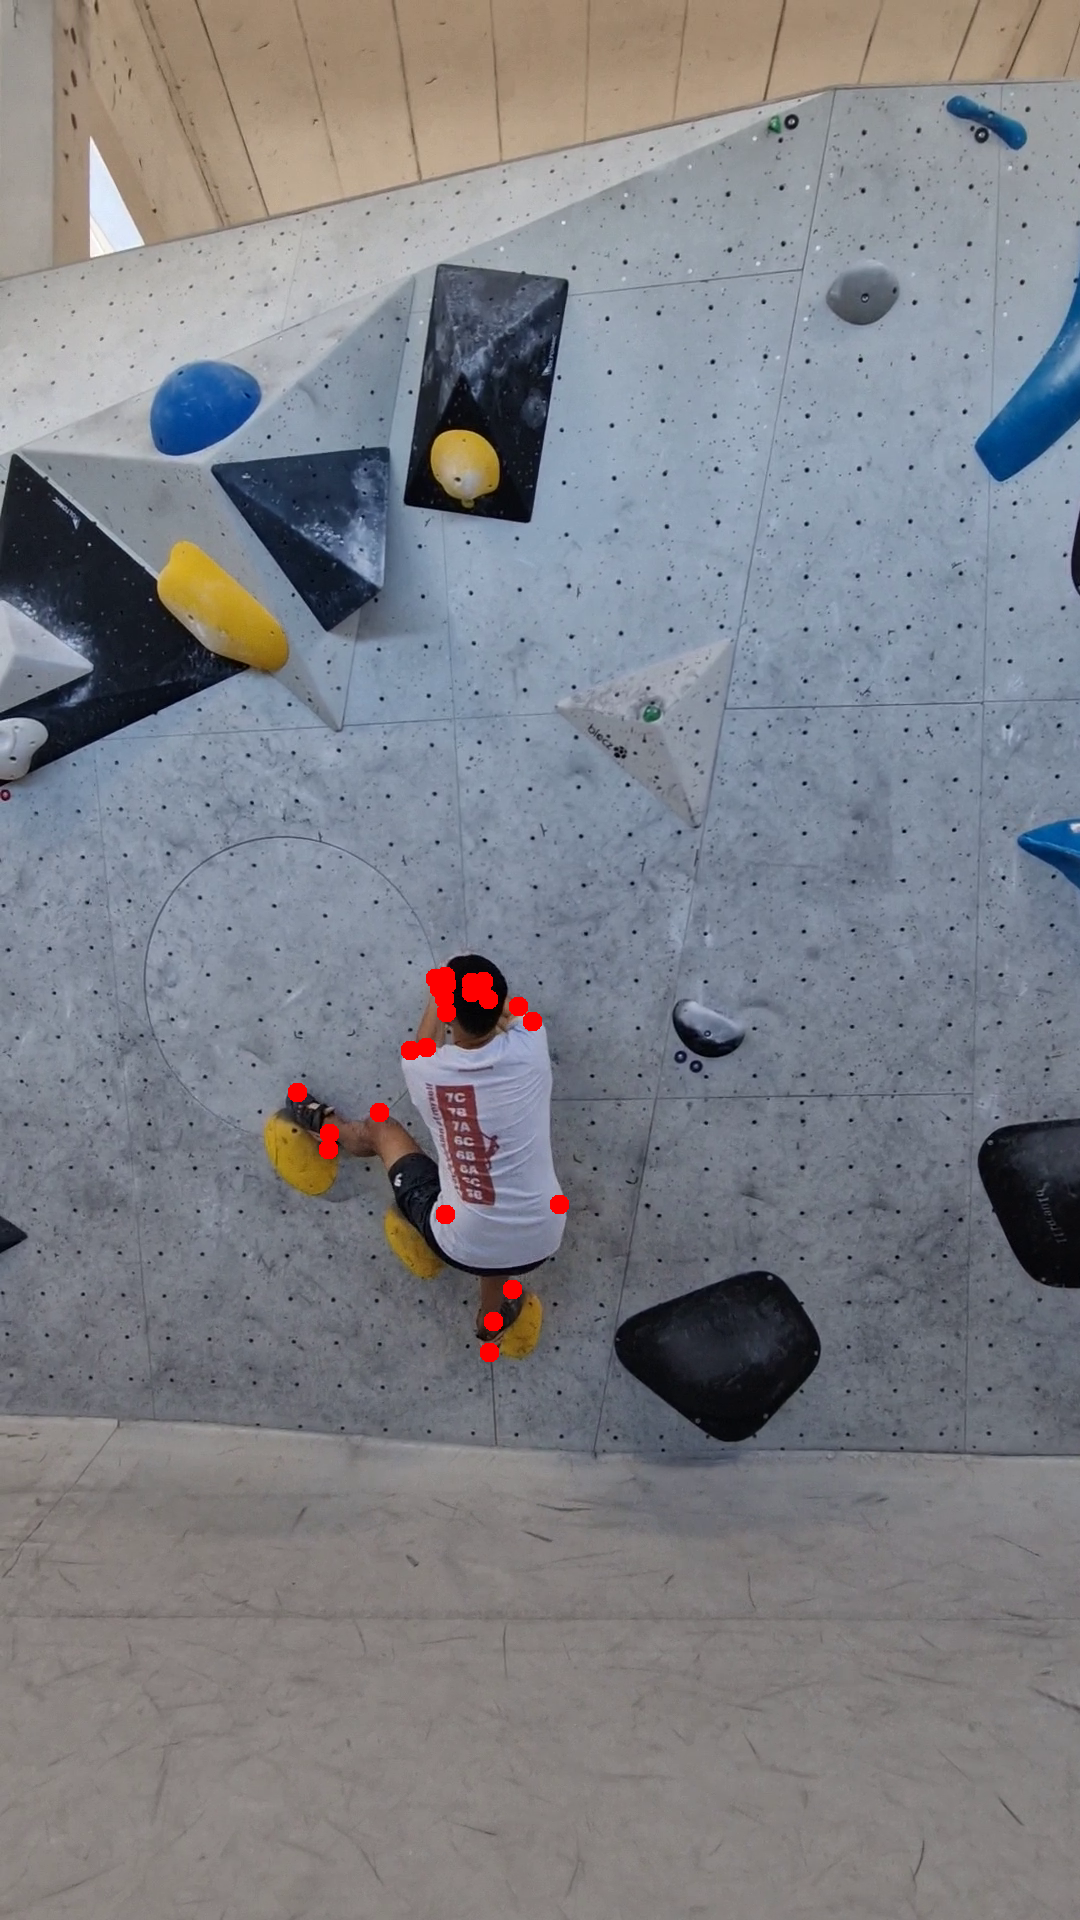
\includegraphics[width=\textwidth]{entities/CA_20.png}
        \caption{Frame 20}
    \end{subfigure}
    \begin{subfigure}{0.3\textwidth}
        \centering
        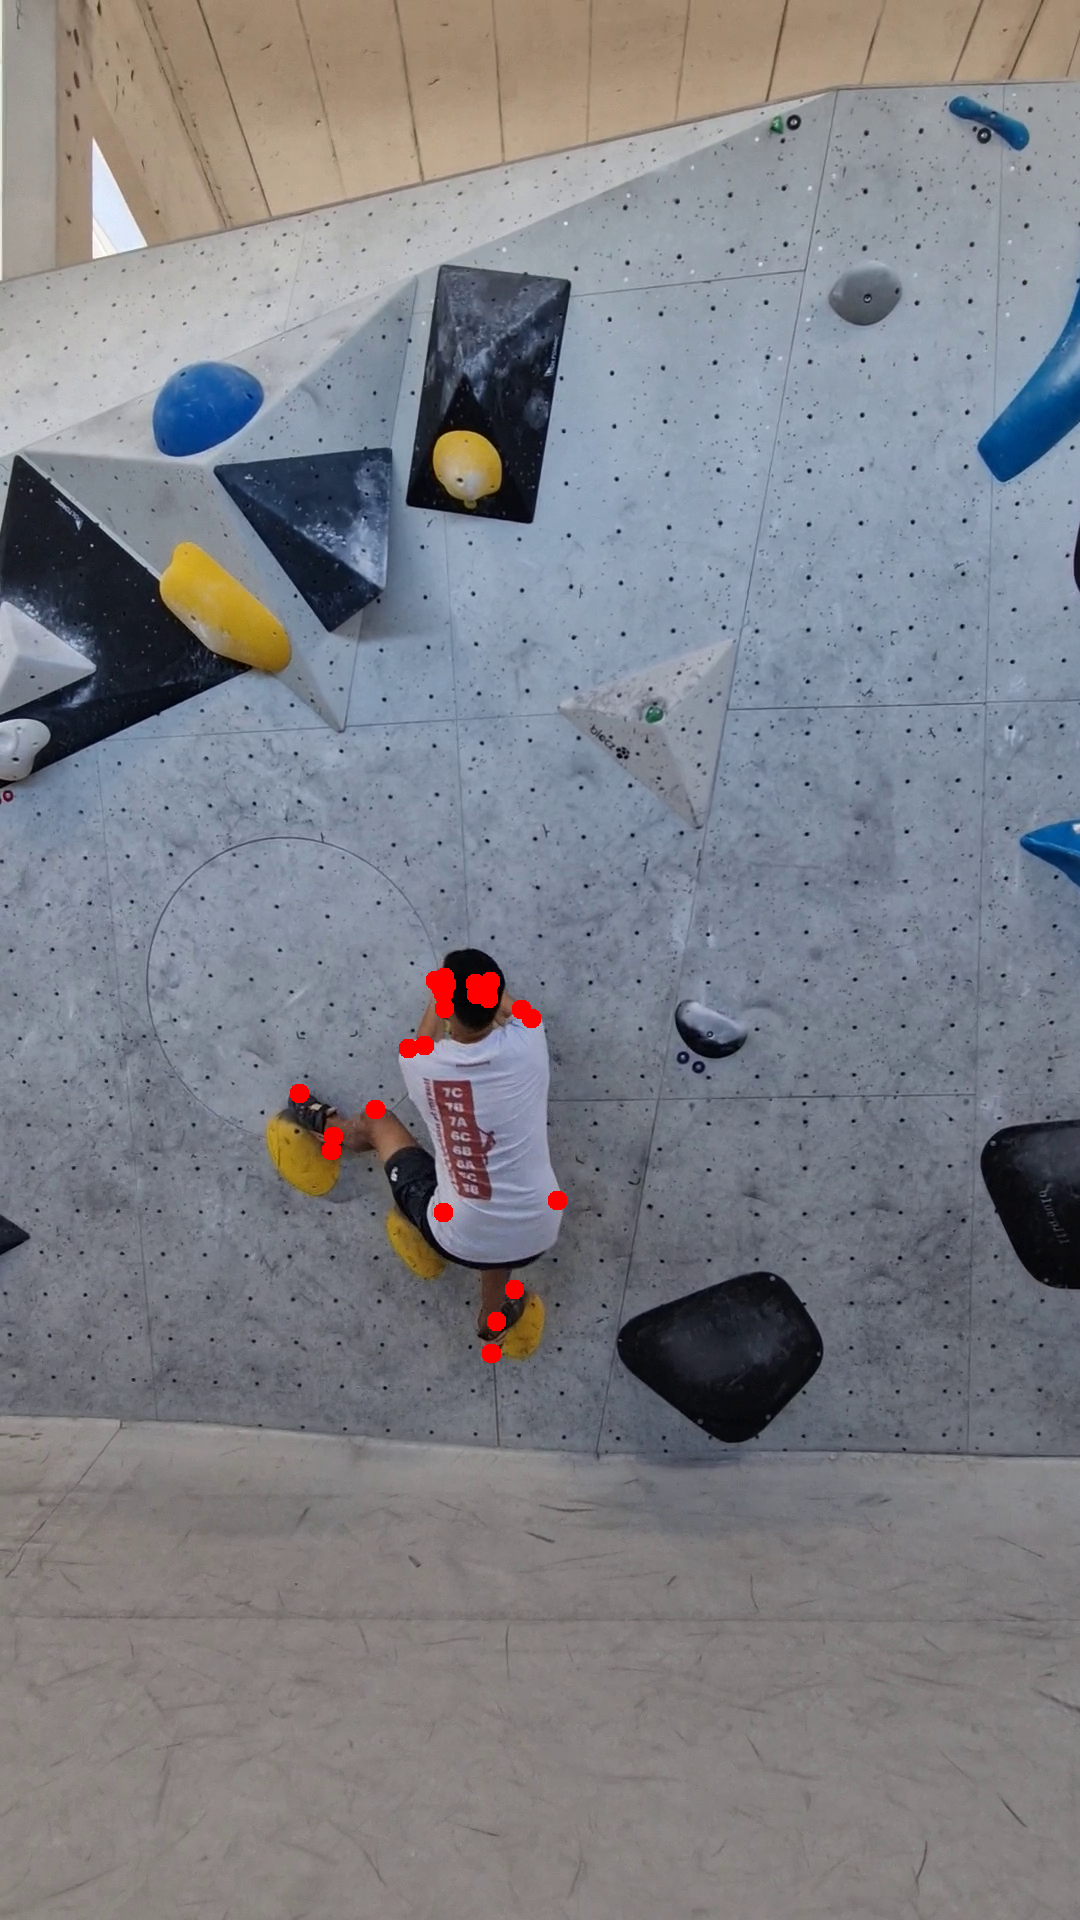
\includegraphics[width=\textwidth]{entities/CA_21.png}
        \caption{Frame 21}
    \end{subfigure}
    \caption{Example of five consecutive frames of a video from the ClimbAlong dataset with the corresponding ground truth keypoints, where the actor holds his position for a while.}
    \label{fig:CA_dataset_static}
\end{figure}

\begin{figure}[htbp]
    \centering
    \begin{subfigure}{0.3\textwidth}
        \centering
        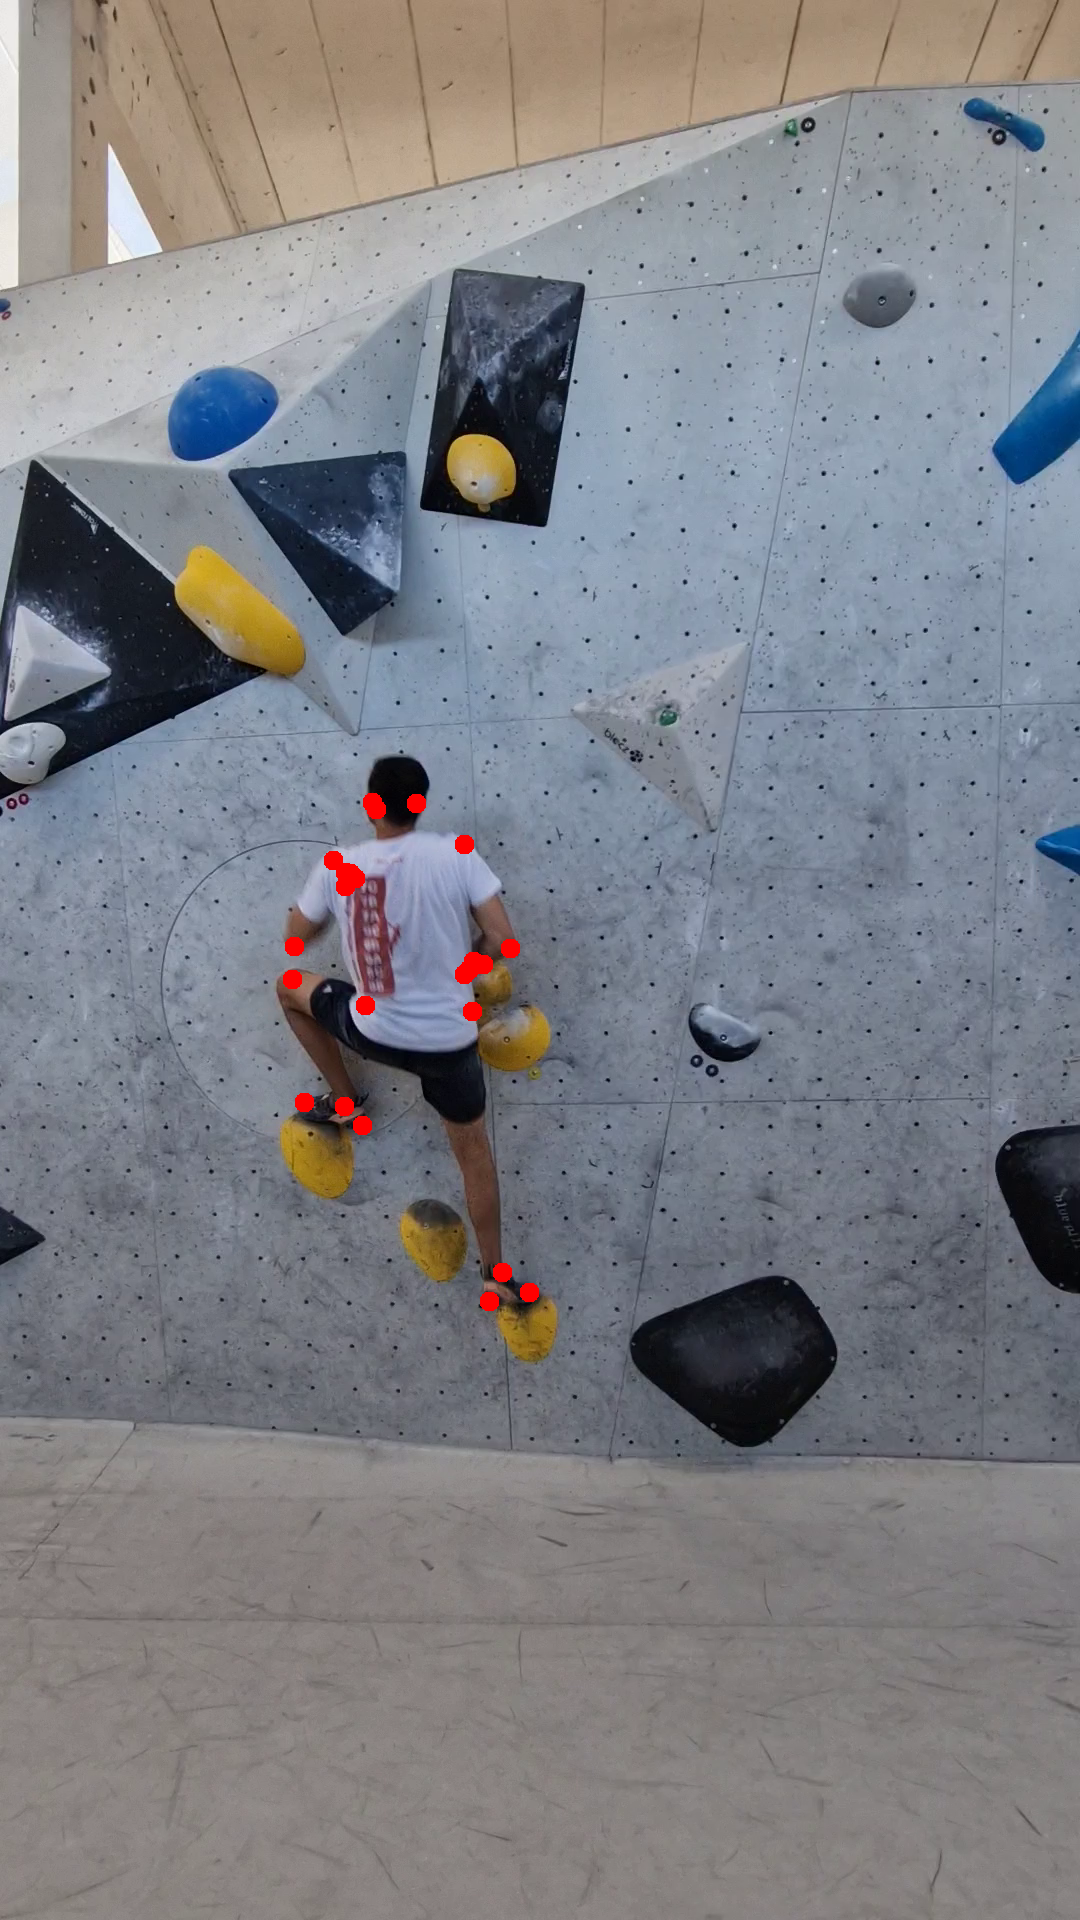
\includegraphics[width=\textwidth]{entities/CA_31.png}
        \caption{Frame 31}
    \end{subfigure}
    \begin{subfigure}{0.3\textwidth}
        \centering
        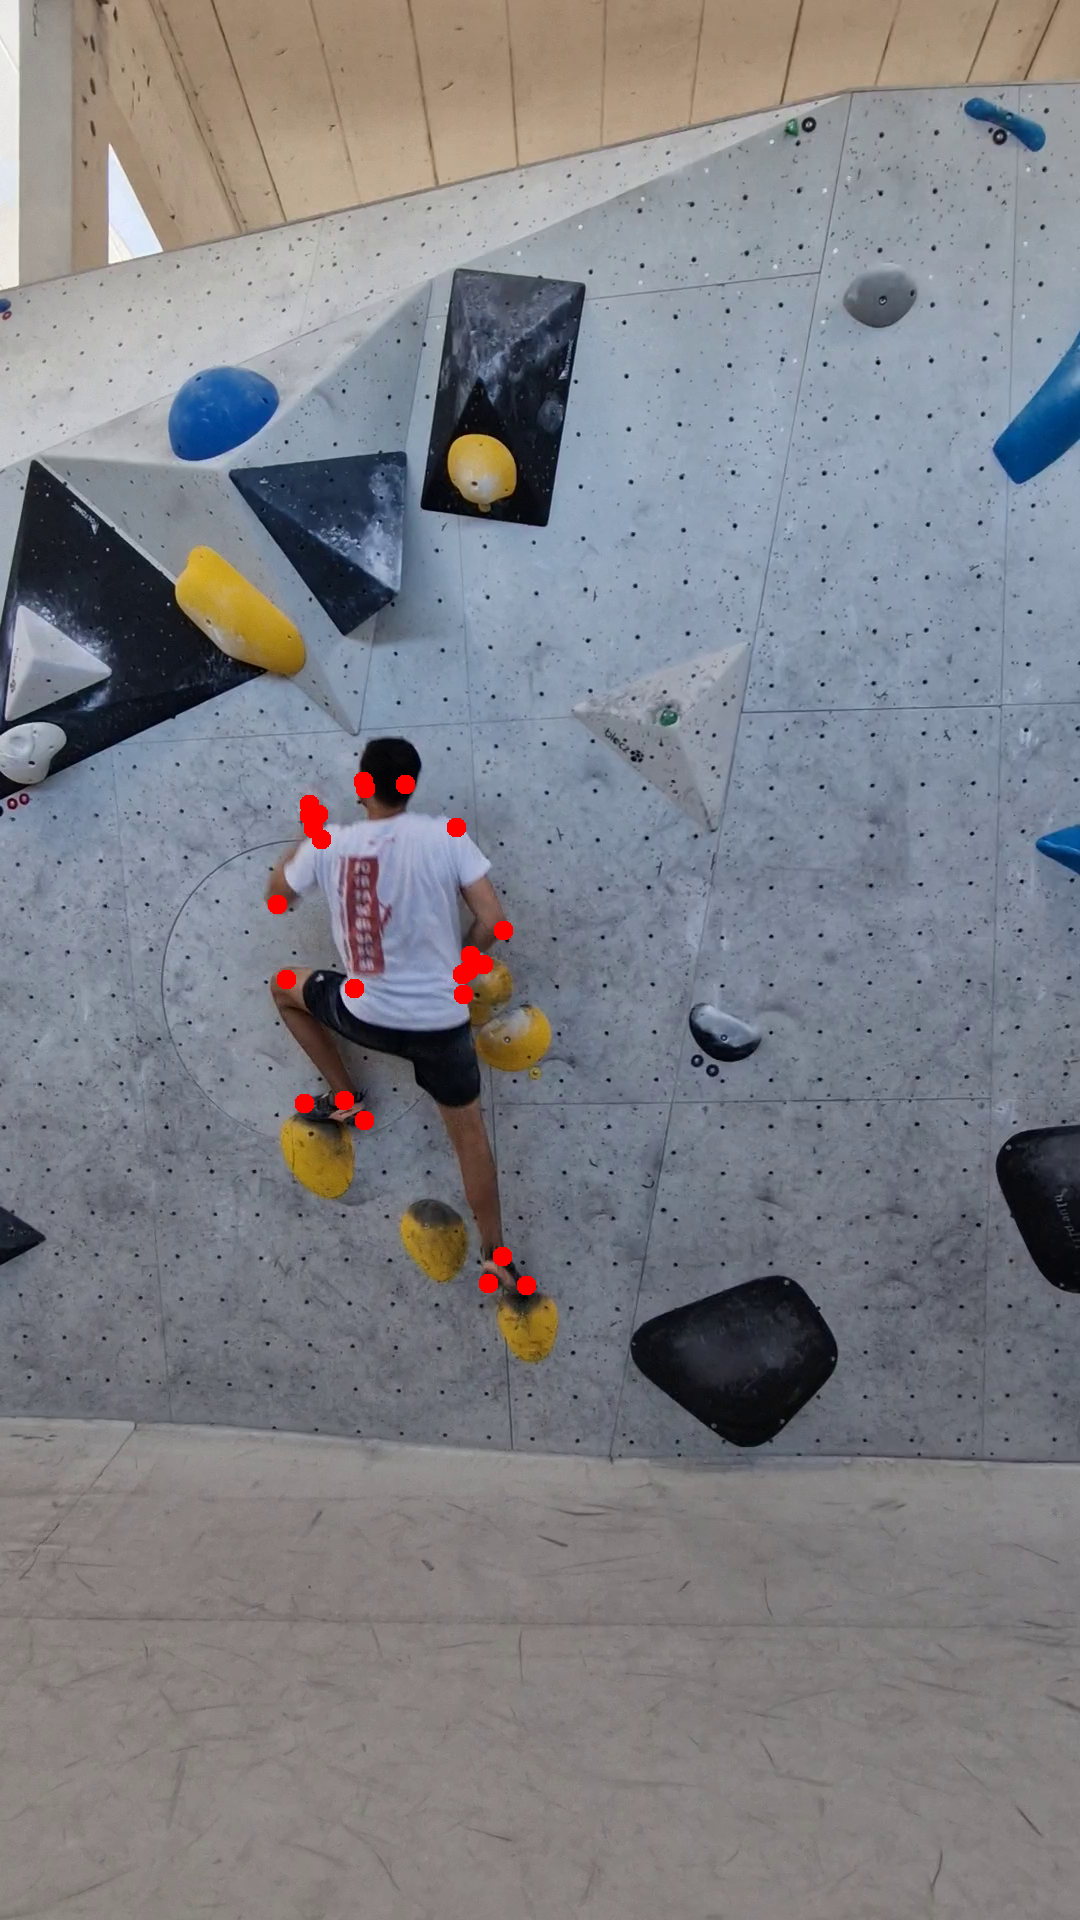
\includegraphics[width=\textwidth]{entities/CA_32.png}
        \caption{Frame 32}
    \end{subfigure}
    \begin{subfigure}{0.3\textwidth}
        \centering
        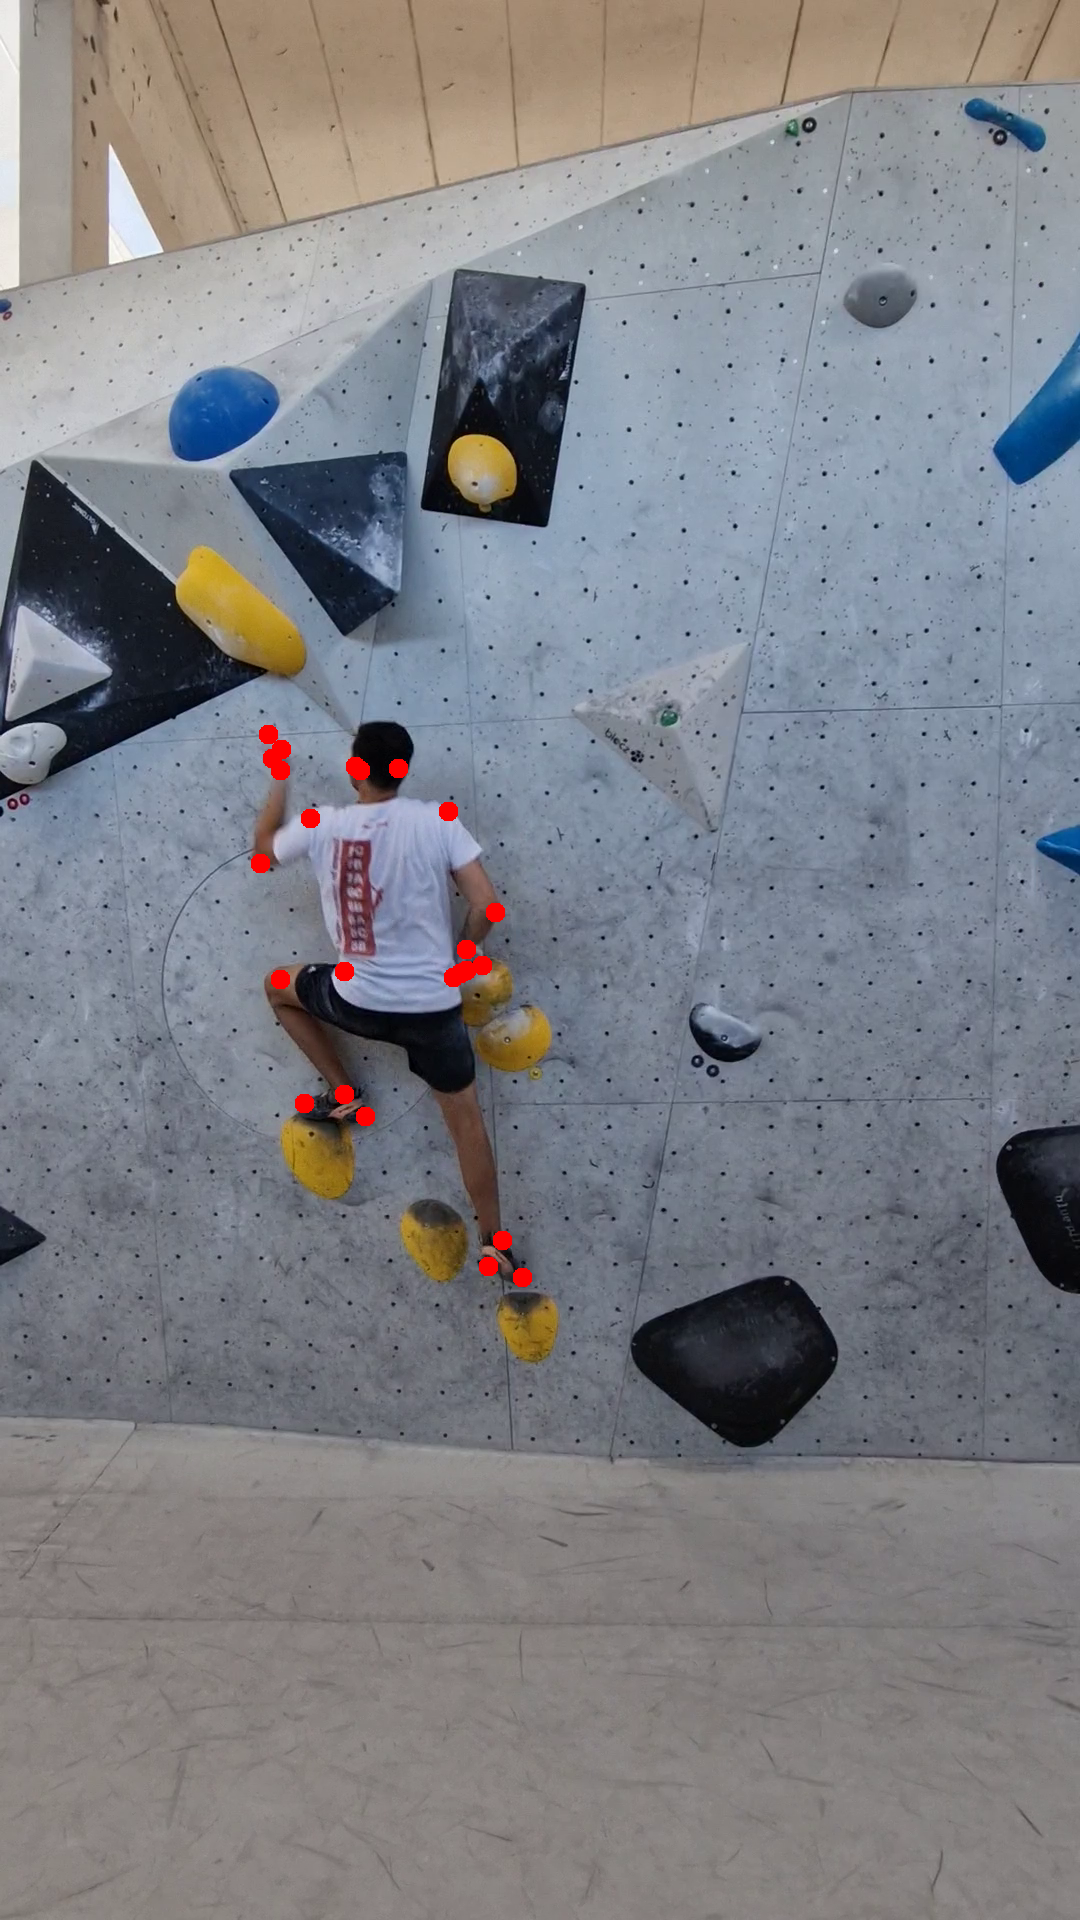
\includegraphics[width=\textwidth]{entities/CA_33.png}
        \caption{Frame 33}
    \end{subfigure}
    \begin{subfigure}{0.3\textwidth}
        \centering
        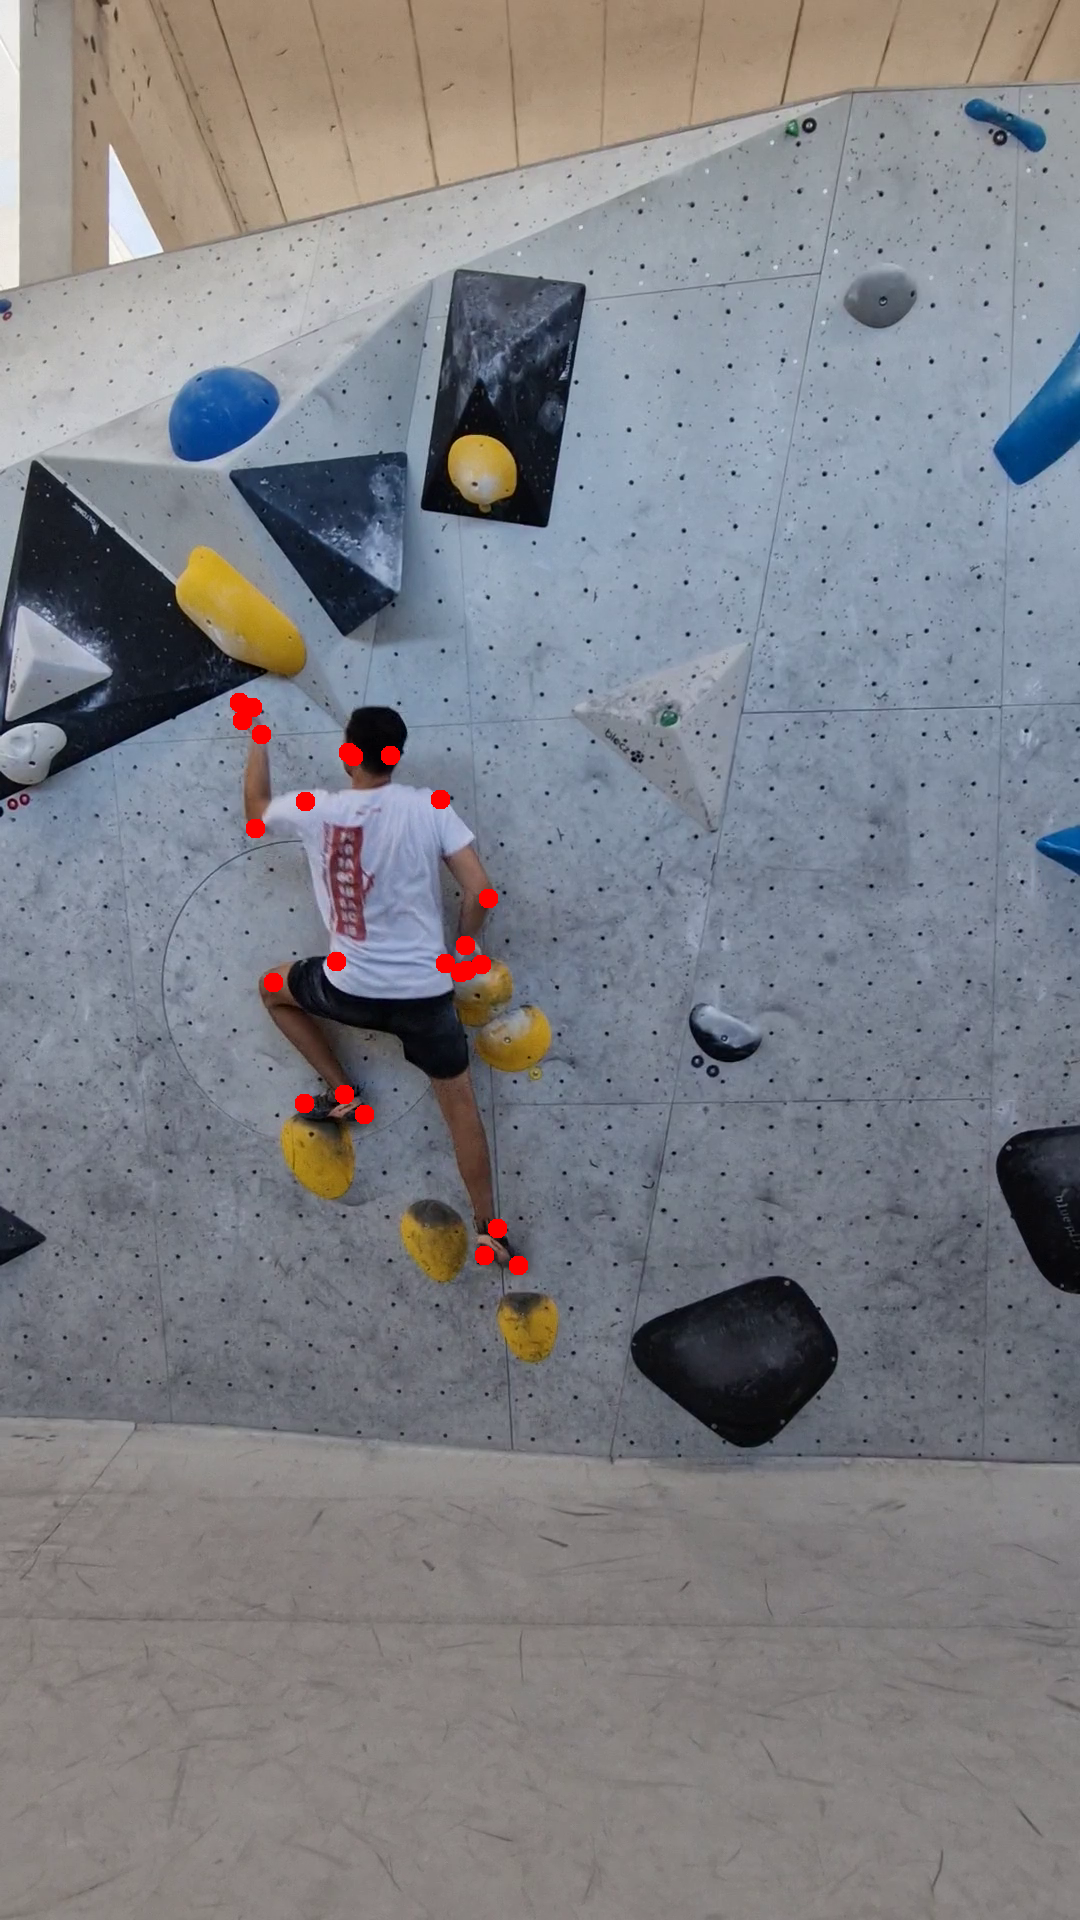
\includegraphics[width=\textwidth]{entities/CA_34.png}
        \caption{Frame 34}
    \end{subfigure}
    \begin{subfigure}{0.3\textwidth}
        \centering
        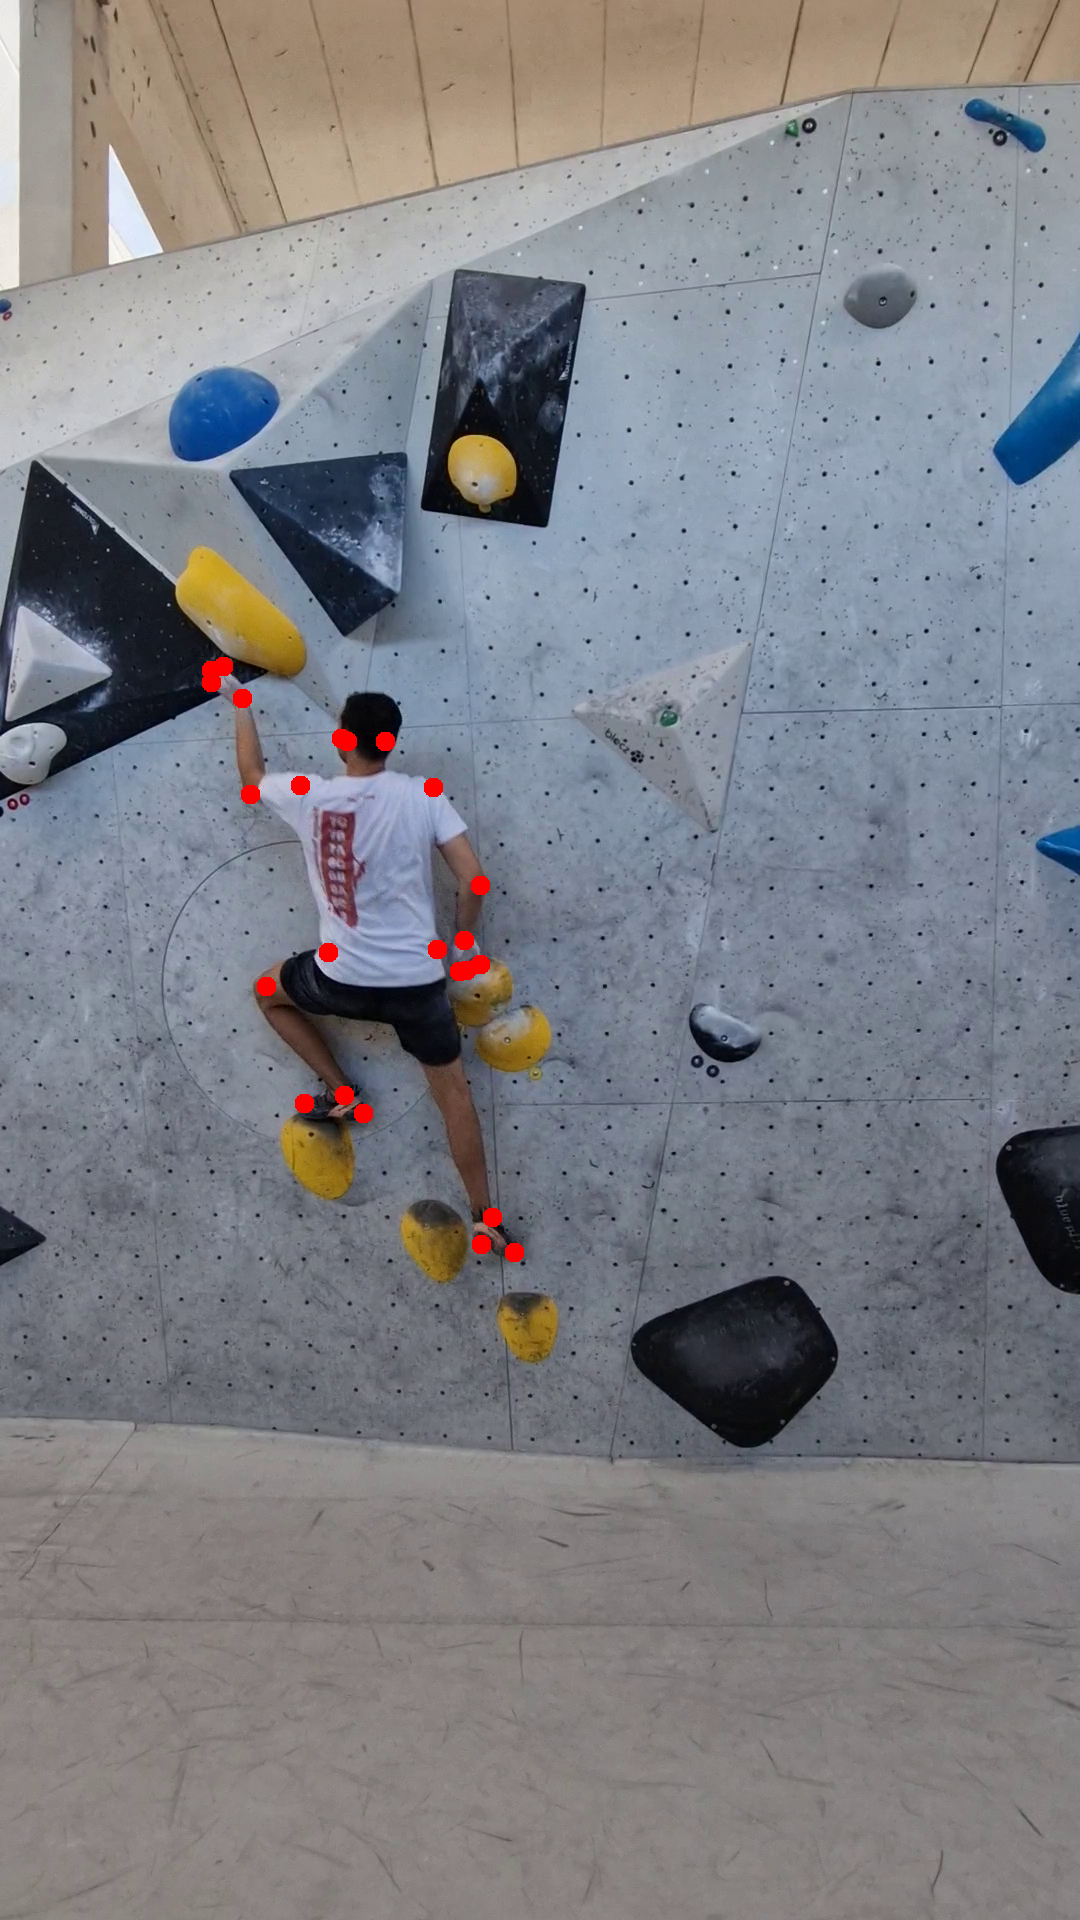
\includegraphics[width=\textwidth]{entities/CA_35.png}
        \caption{Frame 35}
    \end{subfigure}

    \caption{Example of five consecutive frames of a video from the ClimbAlong dataset with the corresponding ground truth keypoints, where the actor performs a quick movement.}
    \label{fig:CA_dataset_quick}
\end{figure}

As the aim of our models is to perform well on climbers, we will be using some annotated data of climbers. For this, ClimbAlong has developed a dataset that we will be using. The dataset consists of videos of various climbers on bouldering walls, where each video contains just a single climber. Figure \ref{fig:CA_dataset_static} and \ref{fig:CA_dataset_quick} illustrates two windows of five consecutive frames of a single video from the ClimbAlong dataset. As shown in the figures, the videos in the dataset contains both static movements, where the climber holds a position for a while, as well as quick movements.
\\
\\
The dataset consists of $30$ fully annotated videos and a total of $10,293$ fully annotated frames, where each annotation consists of $25$ keypoints. Table \ref{tab:keypoints} gives an overview of which keypoints are annotated in the dataset. Each videos is filmed in portrait mode with a resolution of $1080 \times 1920$ and $30$ frames per second. We will throughout this project be referring to this dataset as either the \textbf{ClimbAlong dataset} or the \textbf{finetuning dataset}.

\subsection{The Pretraining Dataset}
\label{sec:dataset_pretraining}
As we will in section \ref{sec:pretraining} be pretraining our models before specializing our models on bouldering, we will be requiring some pretraining data. For this we use the BRACE dataset \cite{BRACE} and parts of the Penn Action dataset \cite{penn_action}. We chose these datasets, as they are rather similar to the ClimbAlong dataset, as they also mostly consist of unusual movements and only very few usual movements, such as walking. Generally, the movements of BRACE tend to be quicker than the movements of ClimbAlong, whereas the movements of Penn Action tend to be of a more similar pace. Thus, by incorporating both BRACE and Penn Action, we should capture both the fast and slow movements of the ClimbAlong dataset. The following section introduces these datasets for pretraining.

\subsubsection{The BRACE Dataset}
\label{sec:BRACE}
\begin{figure}[htbp]
    \centering
    \begin{subfigure}{0.45\textwidth}
        \centering
        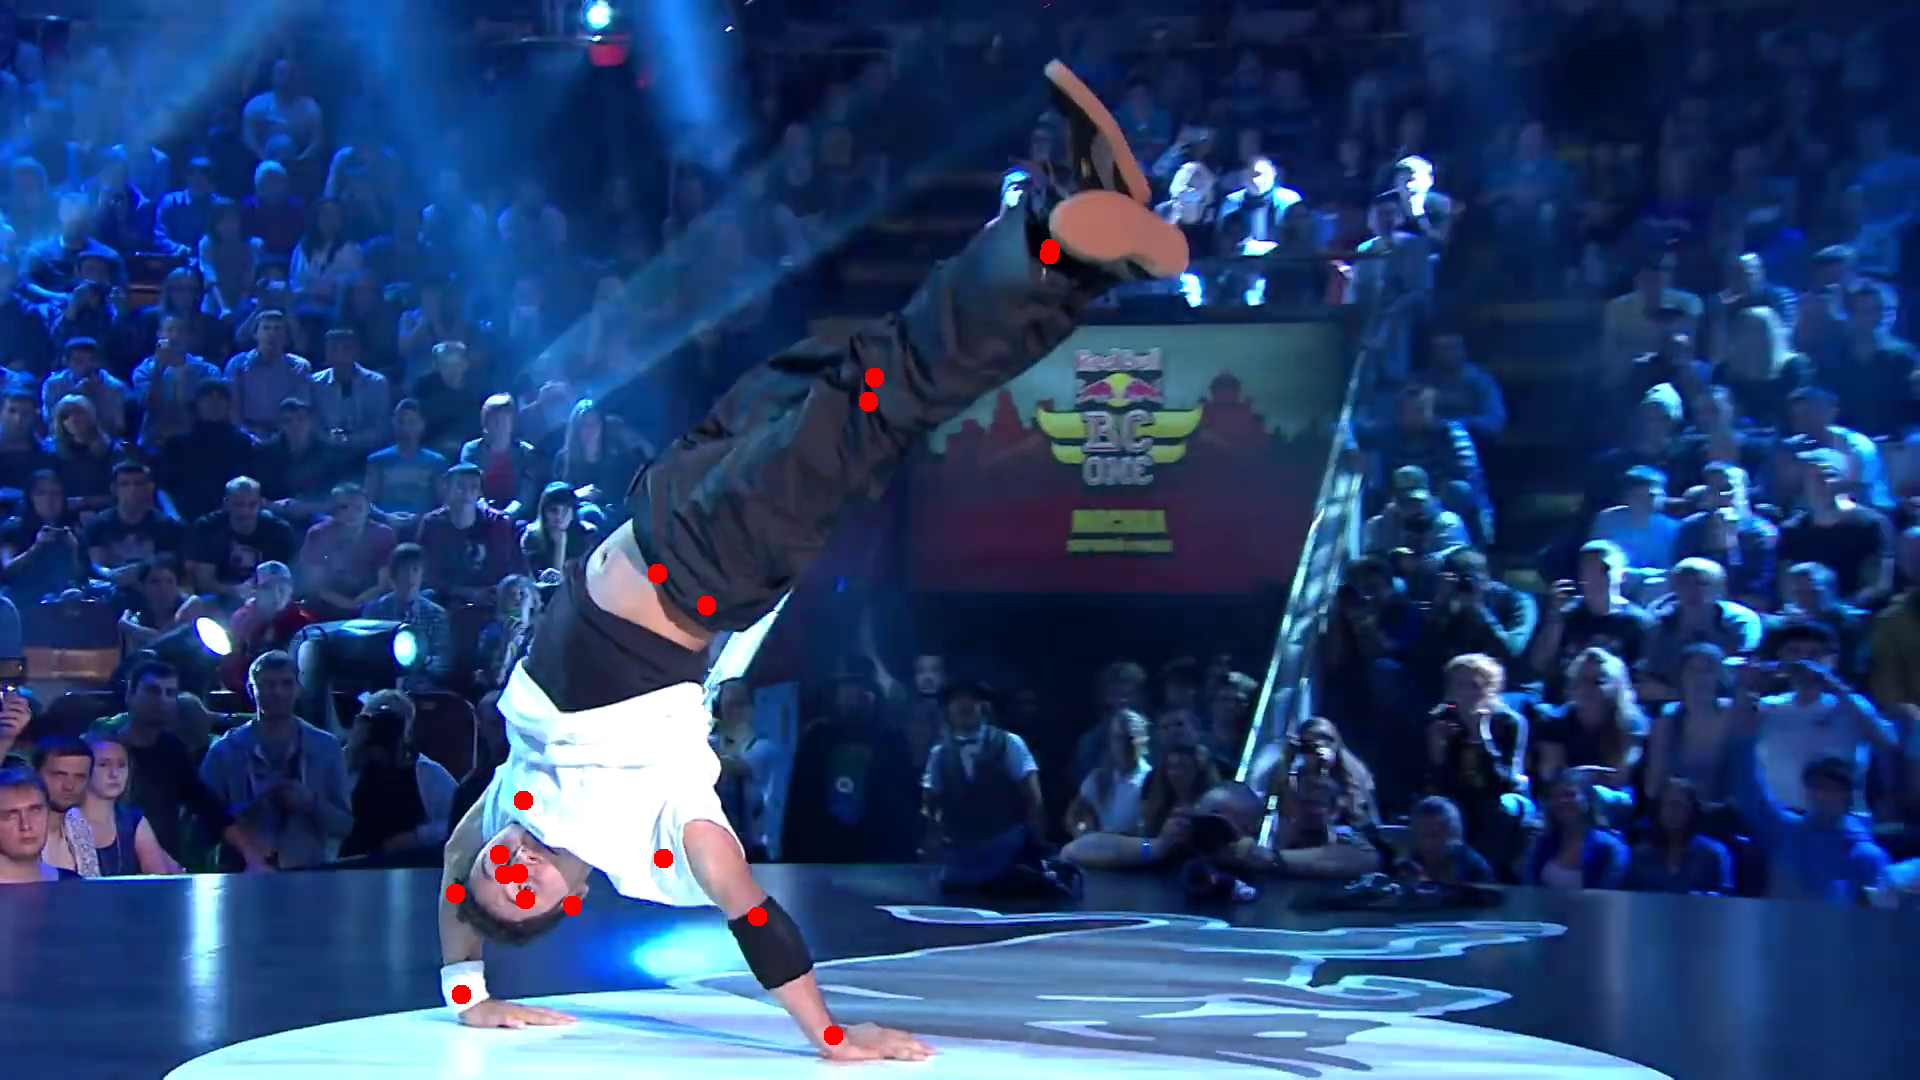
\includegraphics[width=\textwidth]{entities/BRACE_2450.png}
        \caption{Frame 2450}
    \end{subfigure}
    \begin{subfigure}{0.45\textwidth}
        \centering
        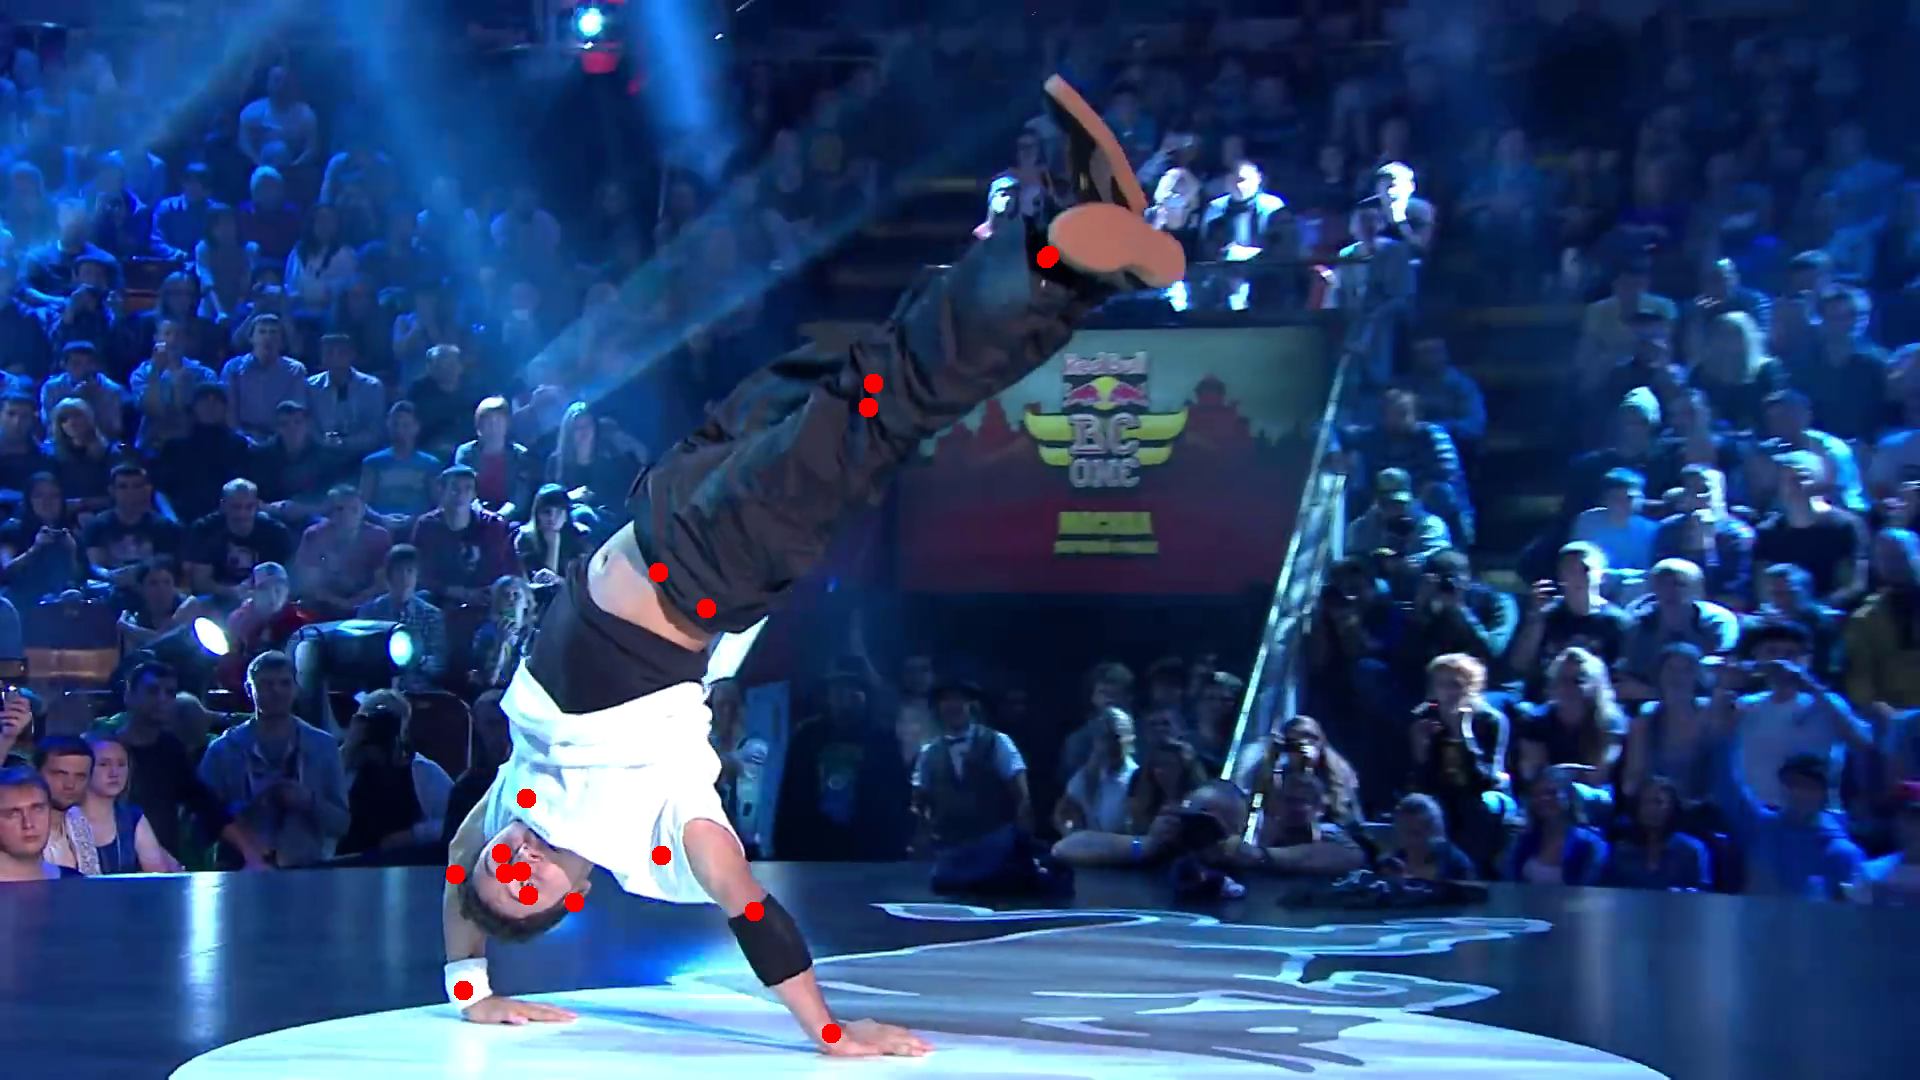
\includegraphics[width=\textwidth]{entities/BRACE_2451.png}
        \caption{Frame 2451}
    \end{subfigure}
    \begin{subfigure}{0.45\textwidth}
        \centering
        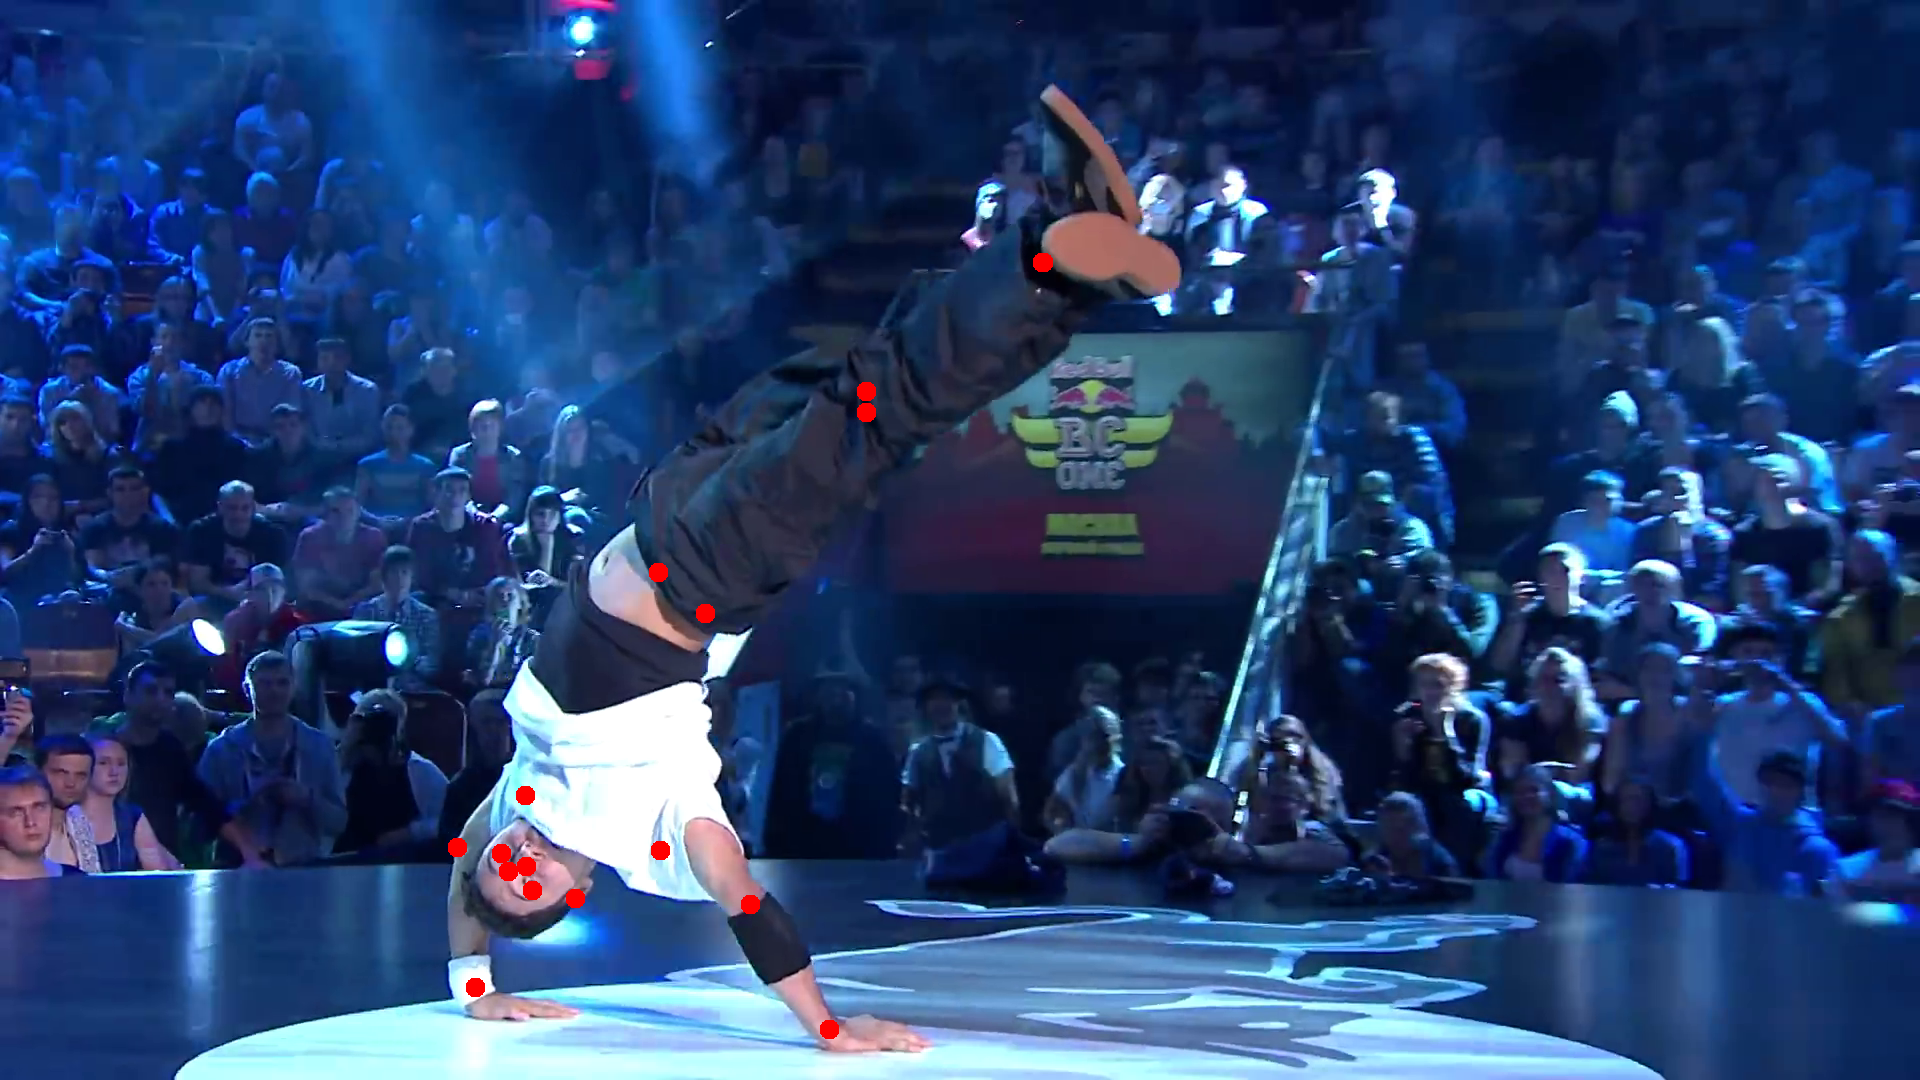
\includegraphics[width=\textwidth]{entities/BRACE_2452.png}
        \caption{Frame 2452}
    \end{subfigure}
    \begin{subfigure}{0.45\textwidth}
        \centering
        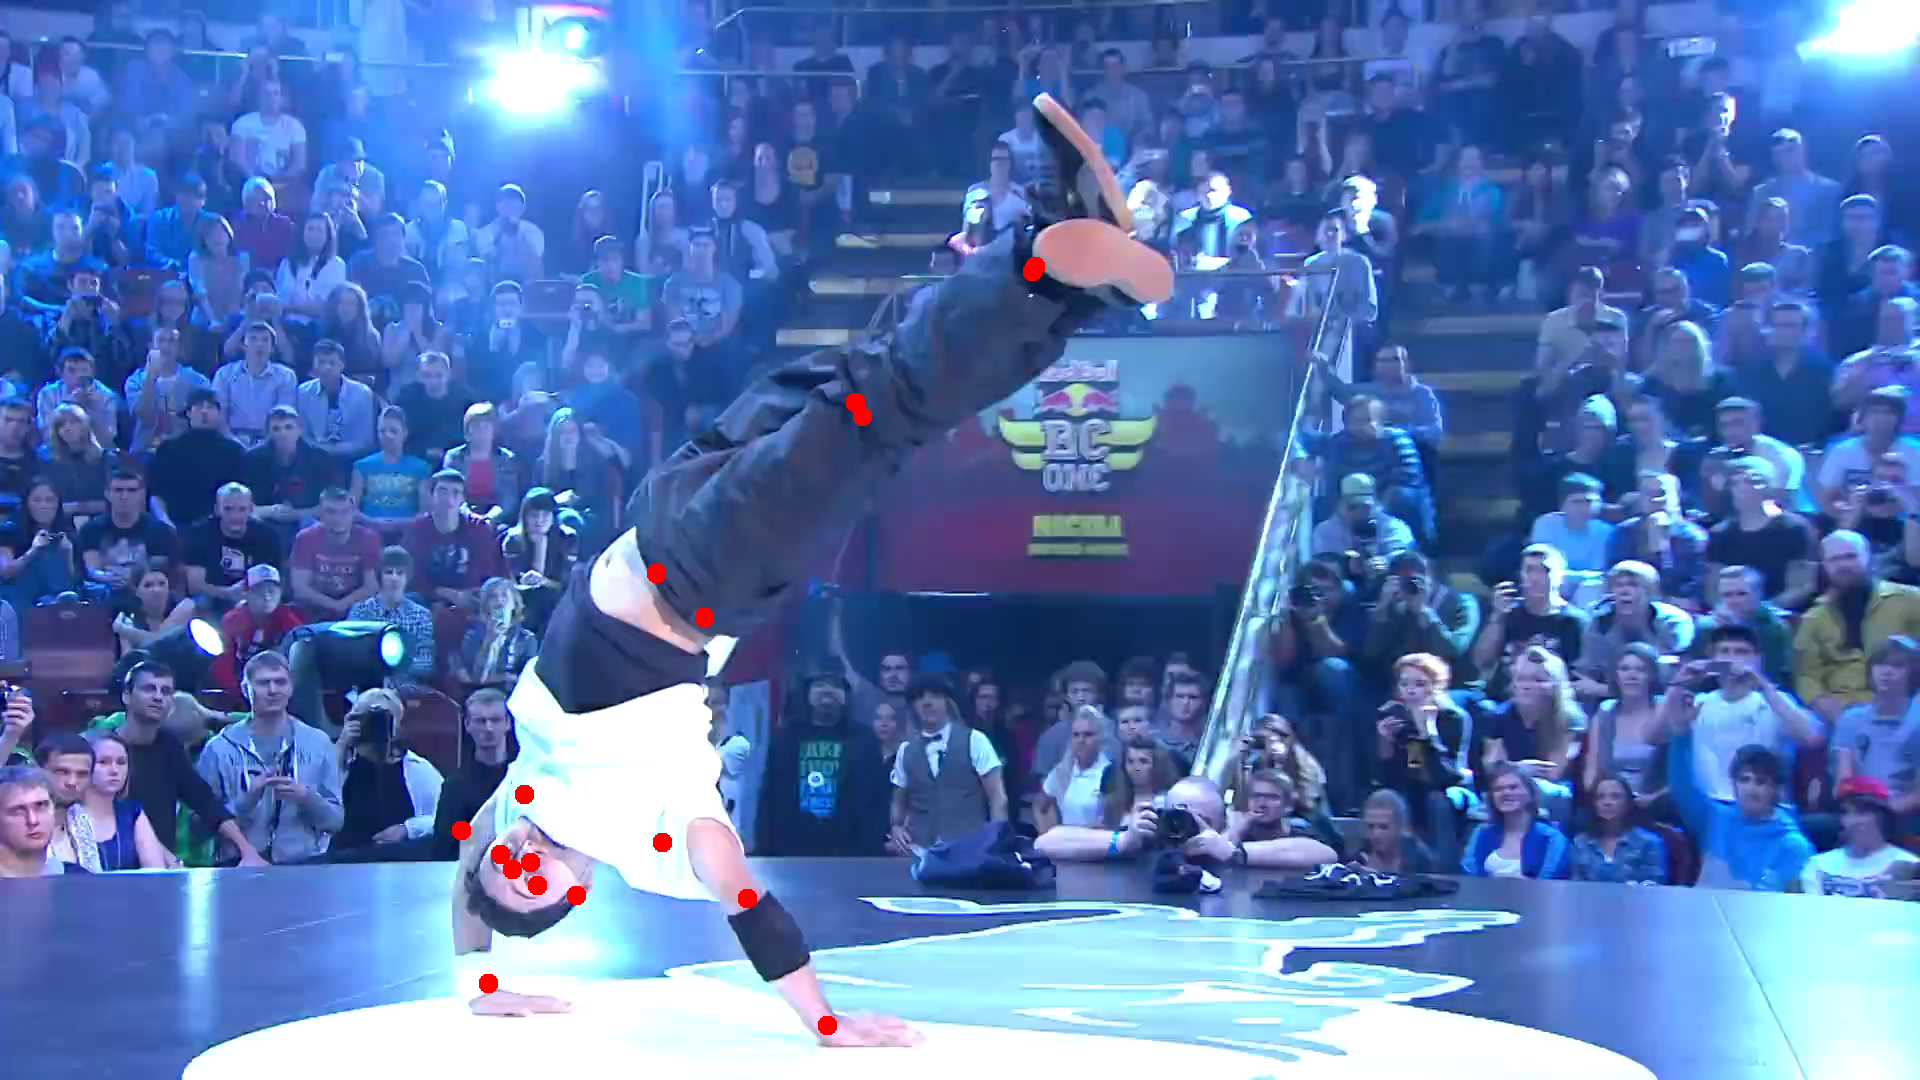
\includegraphics[width=\textwidth]{entities/BRACE_2453.png}
        \caption{Frame 2453}
    \end{subfigure}
    \begin{subfigure}{0.45\textwidth}
        \centering
        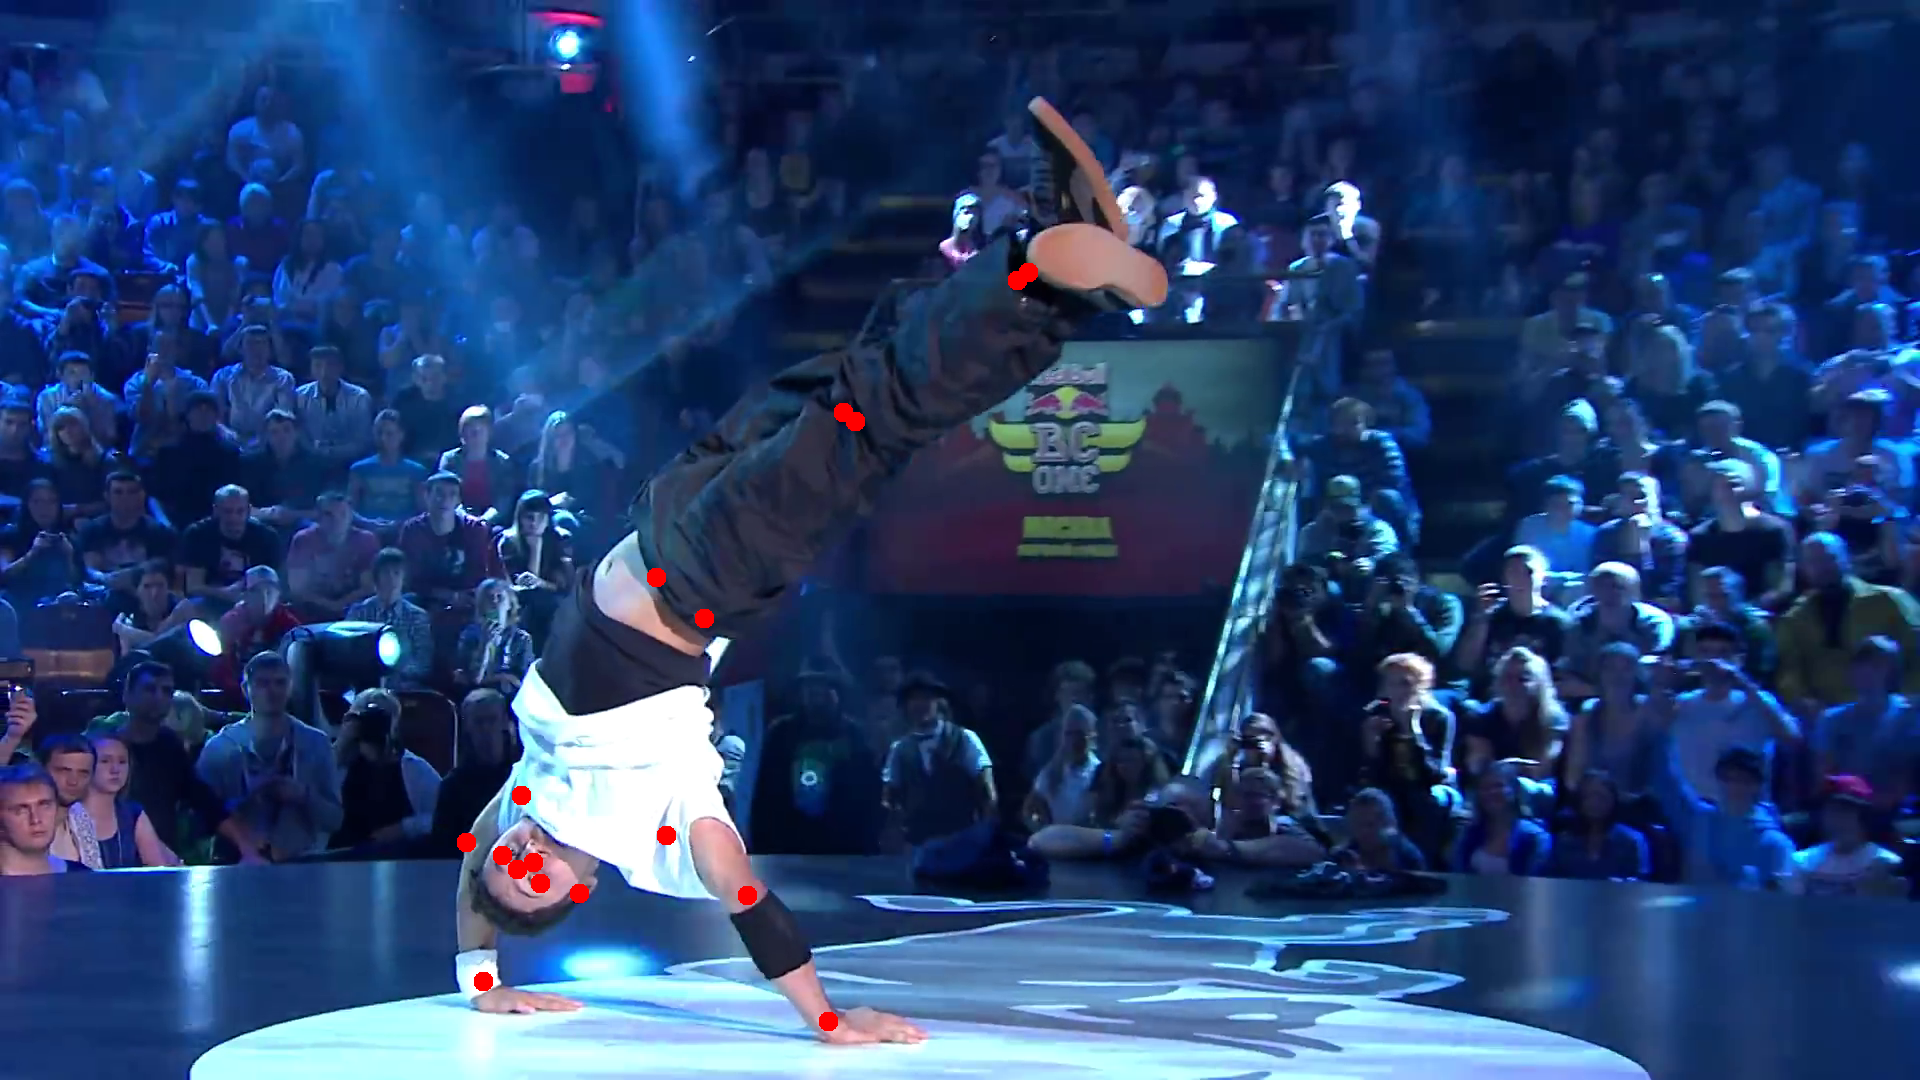
\includegraphics[width=\textwidth]{entities/BRACE_2454.png}
        \caption{Frame 2454}
    \end{subfigure}

    \caption{Example of five consecutive frames of a video from the BRACE dataset with the corresponding ground truth keypoints, where the actor holds his position for a while \cite{BRACE}.}
    \label{fig:BRACE_dataset_static}
\end{figure}

\begin{figure}[htbp]
    \centering
    \begin{subfigure}{0.45\textwidth}
        \centering
        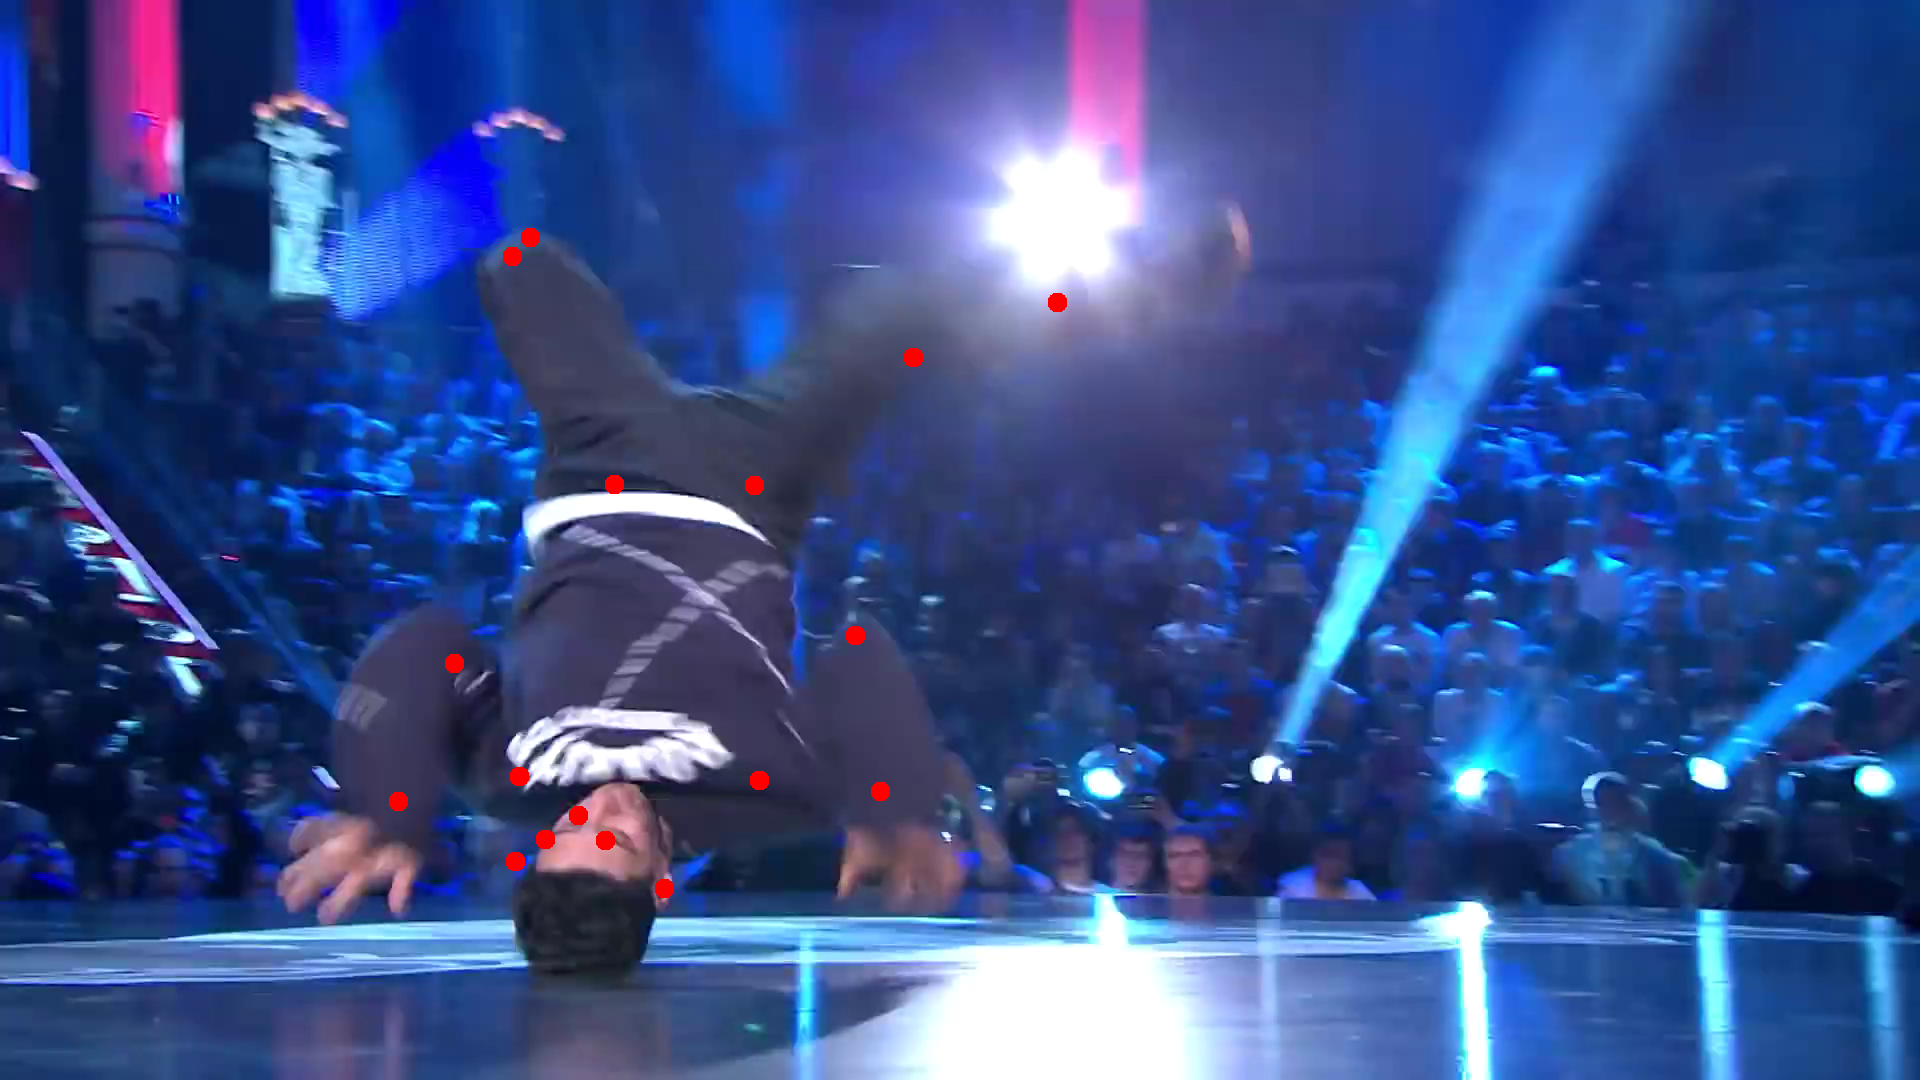
\includegraphics[width=\textwidth]{entities/BRACE_1148.png}
        \caption{Frame 1148}
    \end{subfigure}
    \begin{subfigure}{0.45\textwidth}
        \centering
        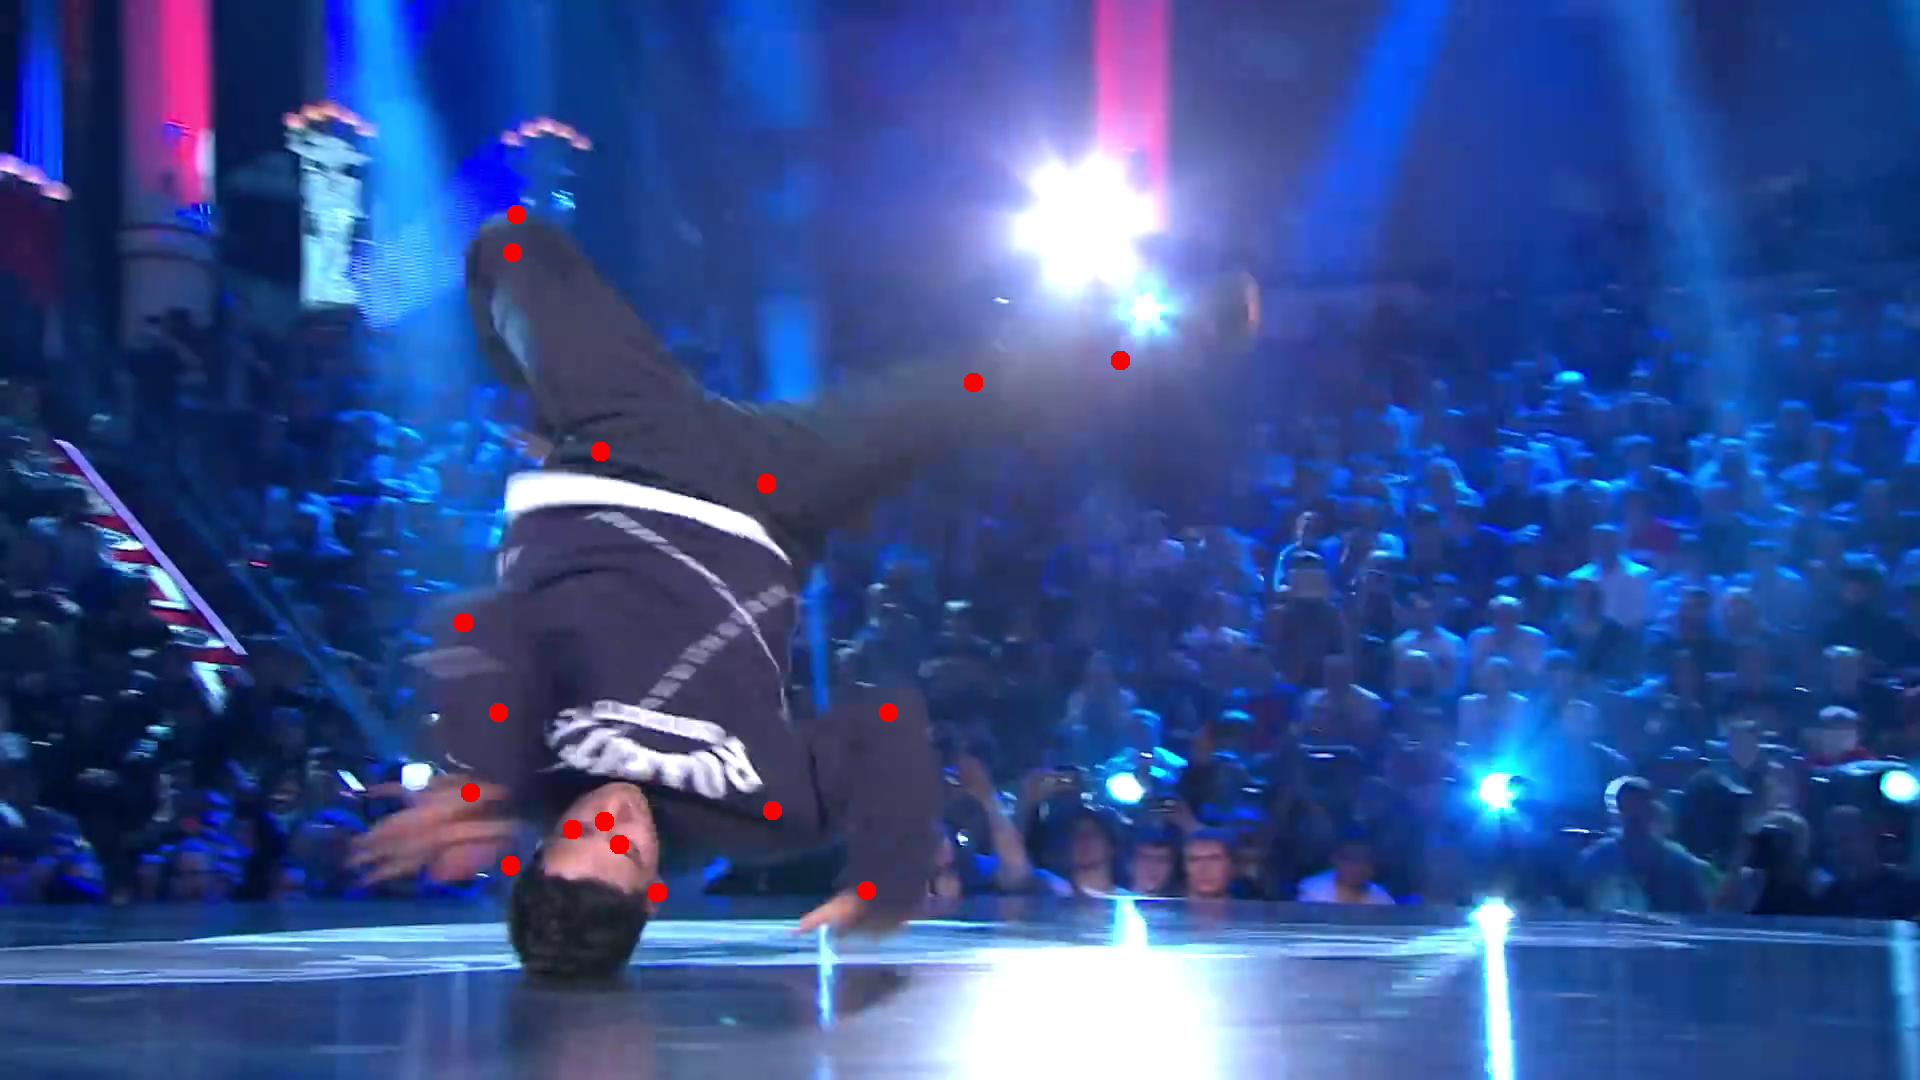
\includegraphics[width=\textwidth]{entities/BRACE_1149.png}
        \caption{Frame 1149}
    \end{subfigure}
    \begin{subfigure}{0.45\textwidth}
        \centering
        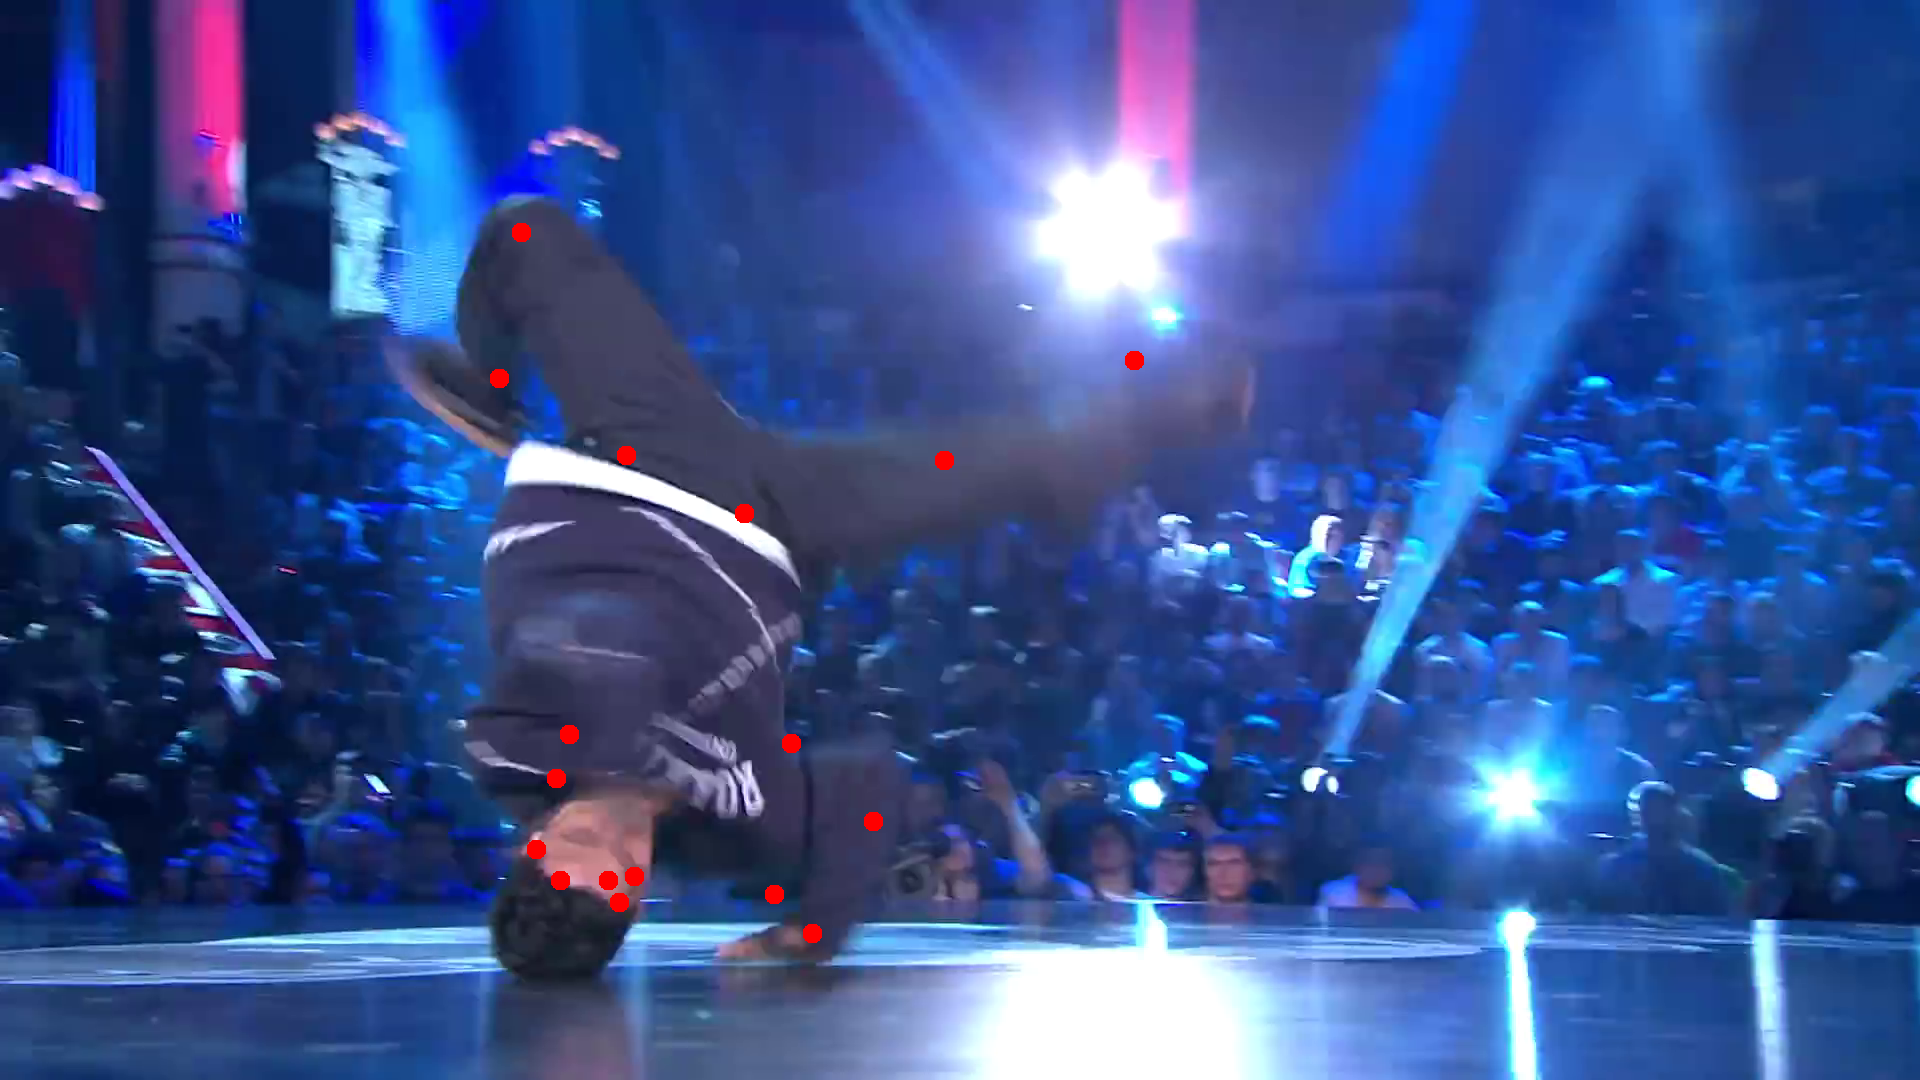
\includegraphics[width=\textwidth]{entities/BRACE_1150.png}
        \caption{Frame 1150}
    \end{subfigure}
    \begin{subfigure}{0.45\textwidth}
        \centering
        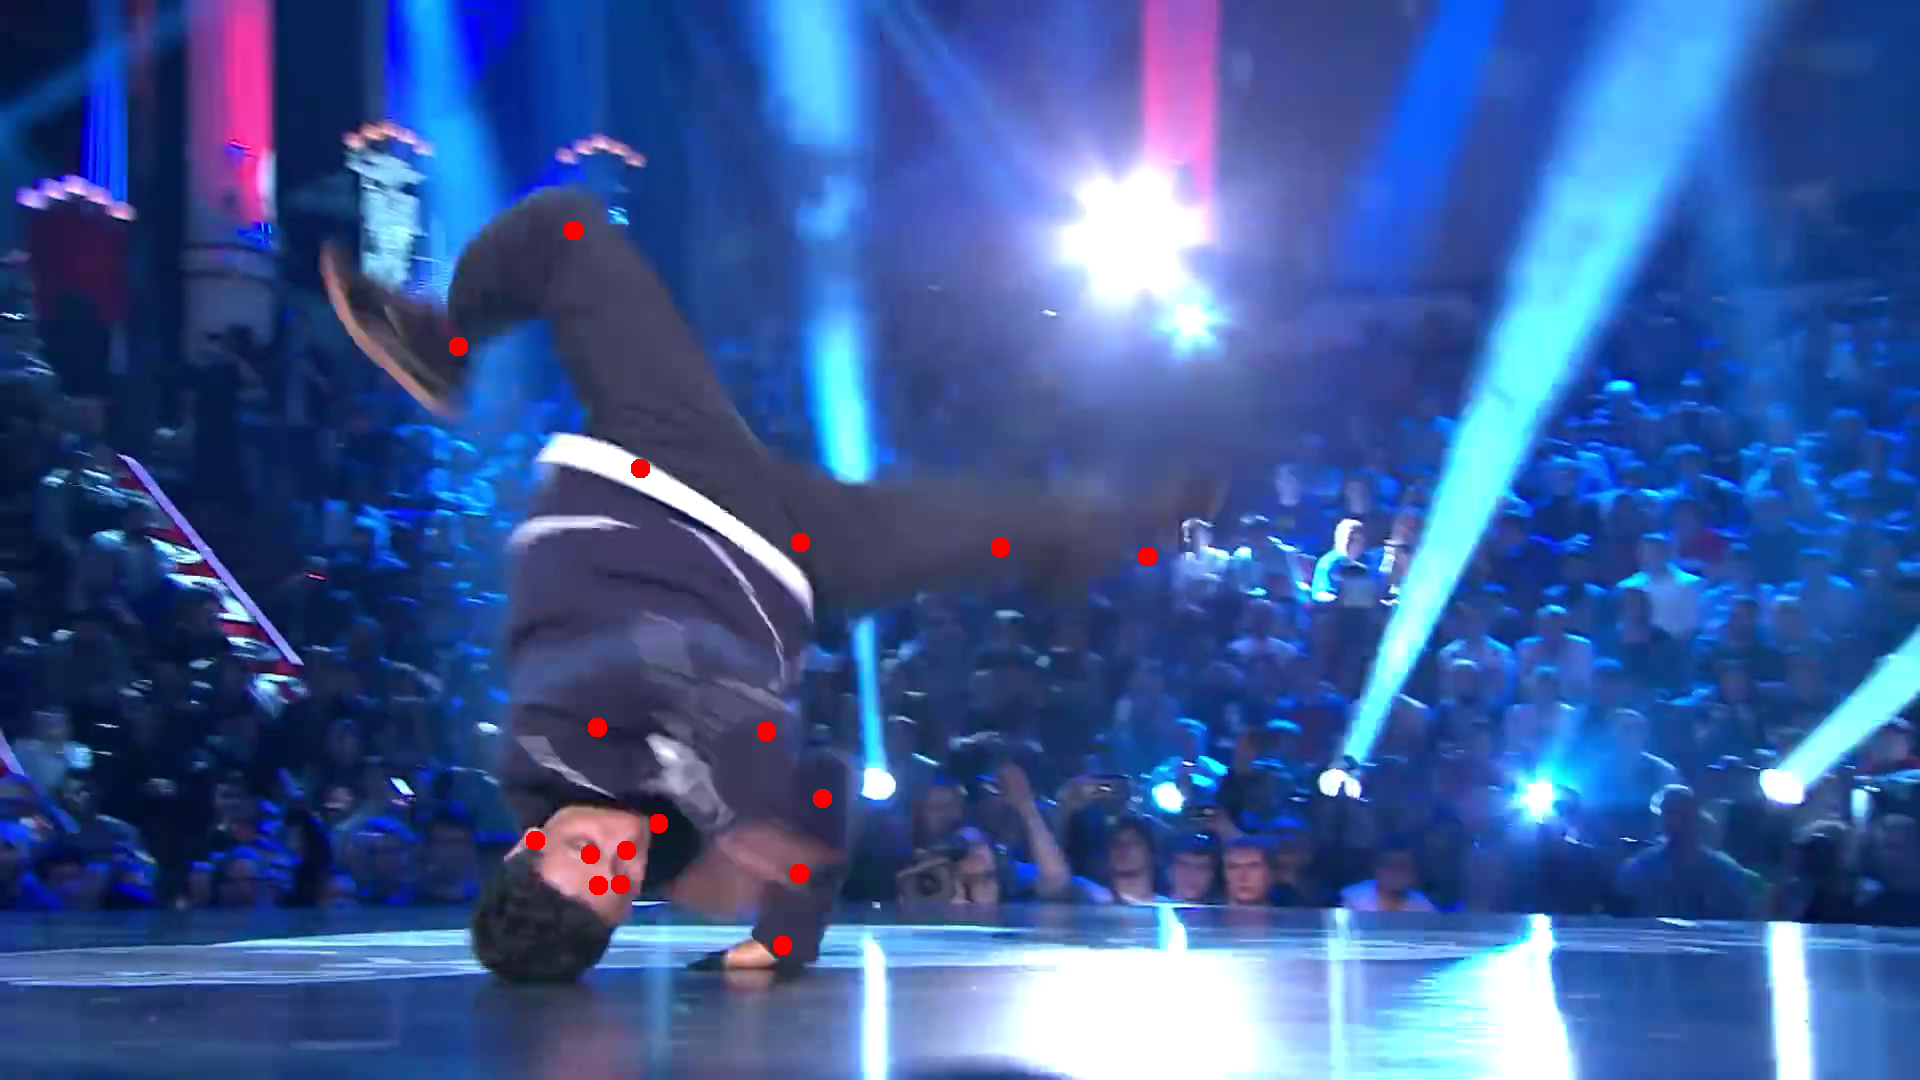
\includegraphics[width=\textwidth]{entities/BRACE_1151.png}
        \caption{Frame 1151}
    \end{subfigure}
    \begin{subfigure}{0.45\textwidth}
        \centering
        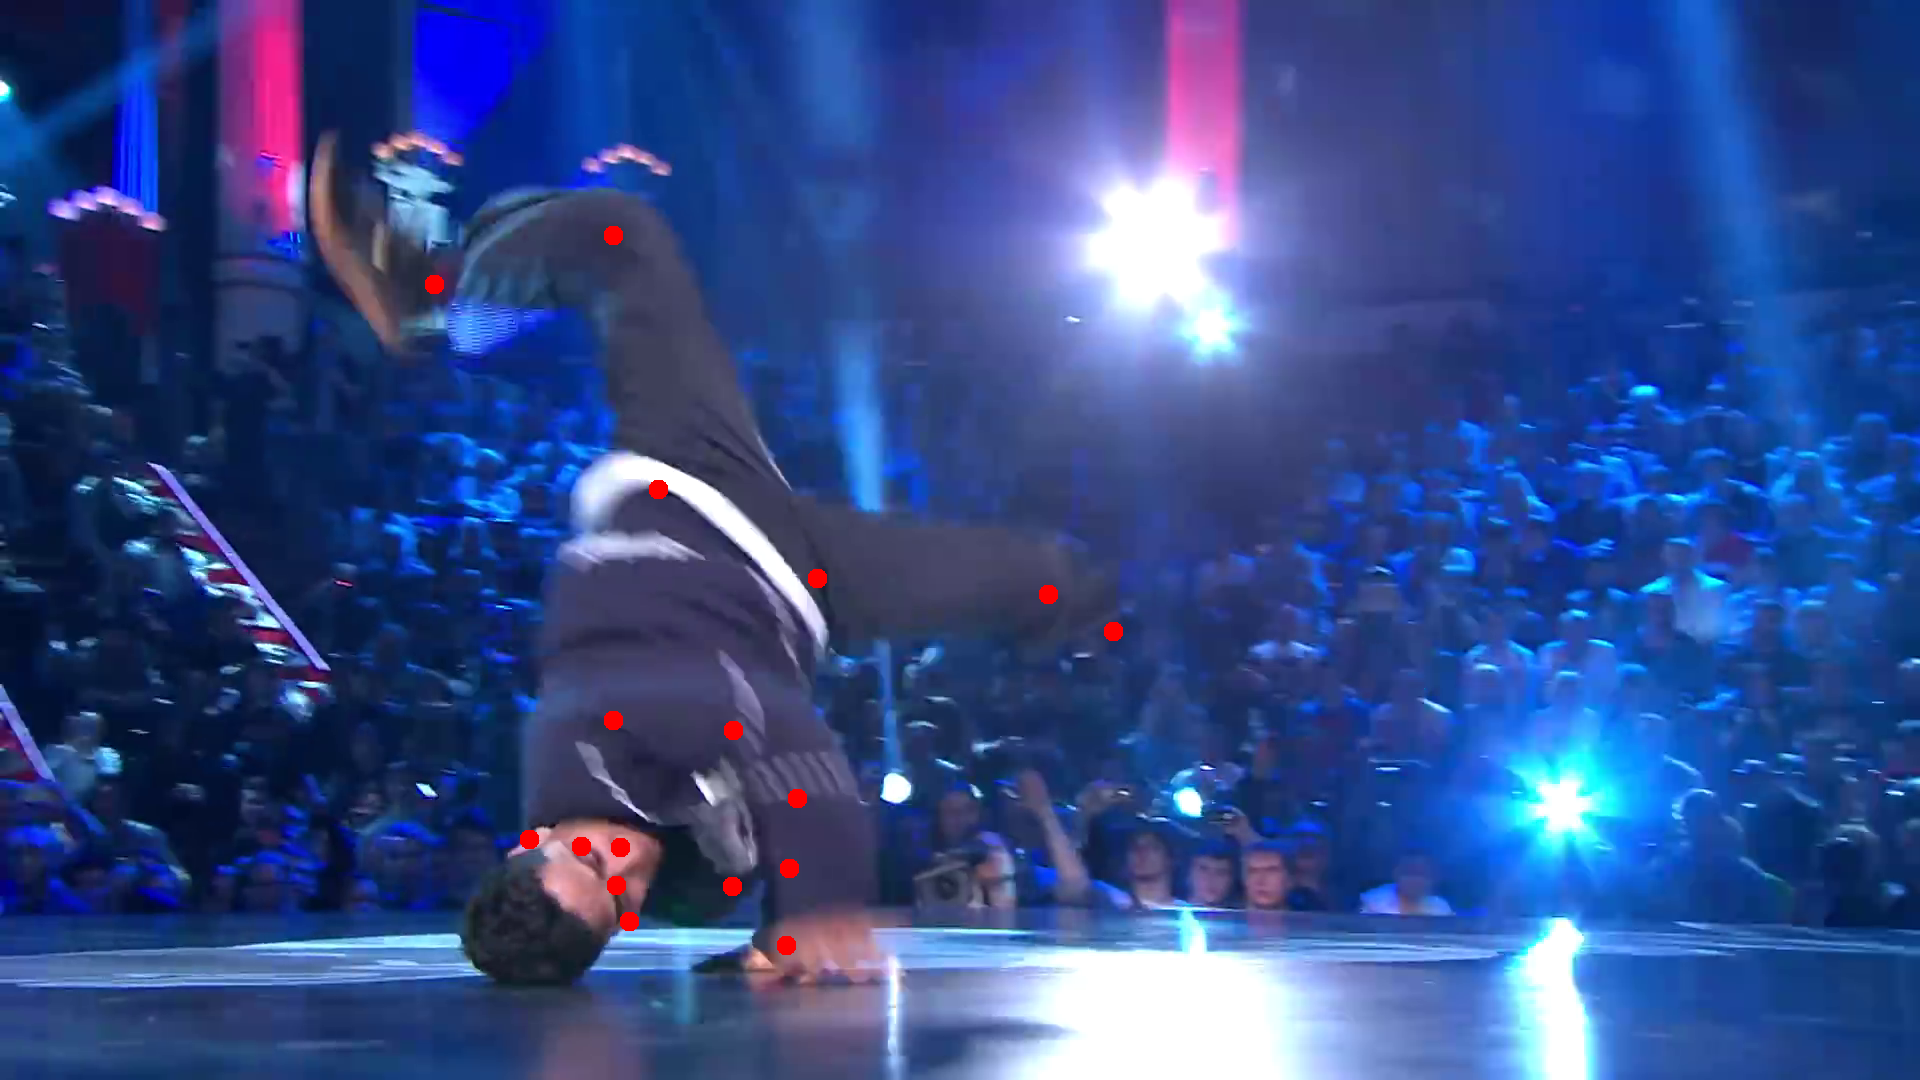
\includegraphics[width=\textwidth]{entities/BRACE_1152.png}
        \caption{Frame 1152}
    \end{subfigure}
    \caption{Example of five consecutive frames of a video from the BRACE dataset with the corresponding ground truth keypoints, where the actor performs a quick movement \cite{BRACE}.}
    \label{fig:BRACE_dataset_quick}
\end{figure}

\noindent The first pretraining dataset we will be using is the BRACE dataset \cite{BRACE}. This dataset consists of $1,352$ video sequences and a total of $334,538$ frames with keypoints annotations of breakdancers. The frames of the video sequences have a resolution of $1920 \times 1080$ \cite{BRACE}.
\\
\\
Generally, the movements of the BRACE dataset are quicker than the movements of the ClimbAlong dataset. Similarly, the annotated person of BRACE tend to swap between static and quick movements just like the annotated person of the ClimbAlong dataset. The static poses of the BRACE dataset tend to occur less frequently than the static poses of the the ClimbAlong dataset, as well as the quick movements tend to be quicker than the quick movements of the ClimbAlong dataset. Figure \ref{fig:BRACE_dataset_static} and \ref{fig:BRACE_dataset_quick} contains two consecutive sequences, each of five frames, that illustrates these two cases.
\\
\\
The frames of the video sequences have been annotated by initially using state-of-the-art human pose estimators. This was then followed by manually annotating outliers, which were detected by a machine learning model. Each frame-annotation consists of $17$ keypoints, as illustrated in Table \ref{tab:keypoints} \cite{BRACE}.

\subsubsection{The Penn Action Dataset}
\label{sec:PA}
\begin{table}
    \begin{tabular}[htbp]{lllllllllllllll}
        \texttt{baseball\_pitch} & \texttt{baseball\_swing} & \texttt{bench\_press} \\
        \texttt{bowling} & \texttt{clean\_and\_jerk} & \texttt{golf\_swing} \\
        \texttt{jumping\_jacks} & \texttt{jump\_rope} & \texttt{pull\_ups} \\
        \texttt{push\_ups} & \texttt{sit\_ups} & \texttt{squats} \\
        \texttt{strumming\_guitar} & \texttt{tennis\_forehand} & \texttt{tennis\_serve}
    \end{tabular}
    \caption{The original $15$ action-types in the Penn Action dataset \cite{penn_action}.}
    \label{tab:PA_actions}
\end{table}

\begin{figure}[htbp]
    \centering
    \begin{subfigure}{0.45\textwidth}
        \centering
        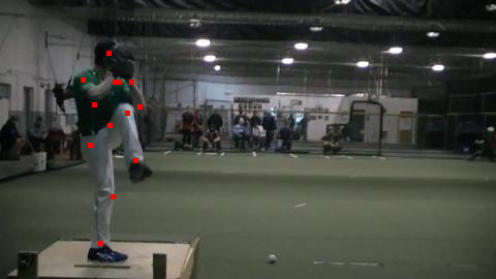
\includegraphics[width=\textwidth]{entities/PA_60.png}
        \caption{Frame 1148}
    \end{subfigure}
    \begin{subfigure}{0.45\textwidth}
        \centering
        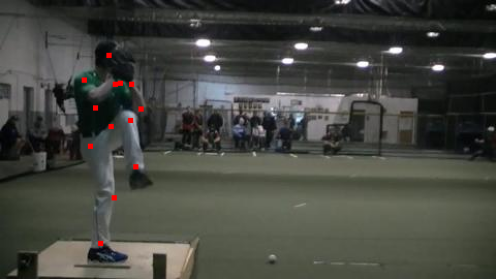
\includegraphics[width=\textwidth]{entities/PA_61.png}
        \caption{Frame 1149}
    \end{subfigure}
    \begin{subfigure}{0.45\textwidth}
        \centering
        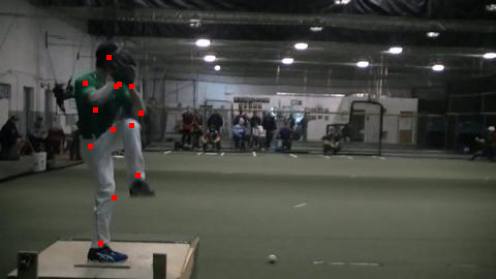
\includegraphics[width=\textwidth]{entities/PA_62.png}
        \caption{Frame 1150}
    \end{subfigure}
    \begin{subfigure}{0.45\textwidth}
        \centering
        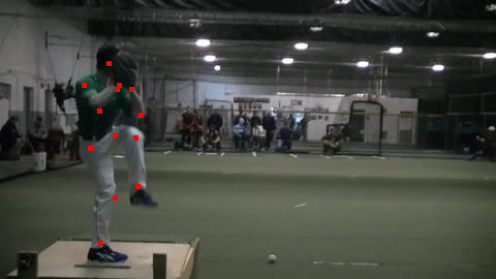
\includegraphics[width=\textwidth]{entities/PA_63.png}
        \caption{Frame 1151}
    \end{subfigure}
    \begin{subfigure}{0.45\textwidth}
        \centering
        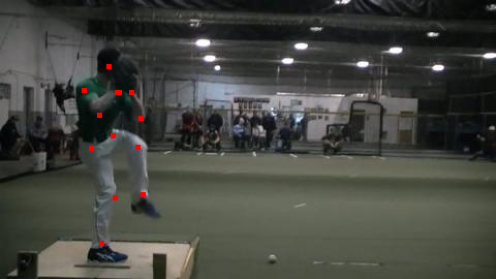
\includegraphics[width=\textwidth]{entities/PA_64.png}
        \caption{Frame 1152}
    \end{subfigure}
    \caption{Example of five consecutive frames of a video from the Penn Action dataset with the corresponding ground truth keypoints \cite{penn_action}.}
    \label{fig:PA_dataset}
\end{figure}
The second pretraining dataset we will be using is the Penn Action dataset \cite{penn_action}. This dataset consists of $2,326$ video sequences of $15$ different action-types. Table \ref{tab:PA_actions} lists these $15$ action-types \cite{penn_action}. Each frame has a resolution within the size of $640 \times 480$ \cite{penn_action}.
\\
\\
Each sequence has been manually annotated, consisting of $13$ joints as well as a corresponding binary visibility-flag for each joint. The handling of the non-visible keypoints is very inconsistent, as the position of some of the keypoints have been estimated, whereas for others it have been placed near one of the corners of the frame \cite{penn_action}.
\\
\\
Unlike the BRACE dataset, most of the poses in the Penn Action dataset are not very unusual and thus are not very relevant for the poses of climbers. For that reason, we have decided to focus on the action-types that may contain more unusual poses. Thus, we only keep the keypoints that have \texttt{baseball\_pitch}, \texttt{bench\_press} or \texttt{sit\_ups} as their corresponding action-type \cite{penn_action}.
\\
\\
In total, we use $307$ video sequences from the Penn Action dataset, consisting of a total of $26,036$ frames. Figure \ref{fig:PA_dataset} illustrates five consecutive frames with its ground truth annotations for one of these video sequences \cite{penn_action}.

\end{document}